\documentclass[a4paper,12pt]{report} %,draft,openright

\usepackage{polski}
\usepackage[utf8]{inputenc} 
\usepackage{gensymb}
\usepackage{textcomp}
\usepackage{tikz}
\usepackage{icomma}
\usepackage{epsf,graphicx}
\usepackage{float}
\usepackage{listings}
\usepackage{subcaption}
\usepackage{latexsym,amssymb}
\usepackage{setspace}
\usepackage[hidelinks]{hyperref}
\usepackage[noadjust]{cite}
\usepackage{indentfirst}
\usepackage{mathtools}
\usepackage[justification=centering]{caption}
\usepackage{multirow}
\newcommand{\nm}{\,\mathrm{nm}}
\newcommand{\um}{\,\mathrm{\mu m}}
\newcommand{\fs}{\,\mathrm{fs}^2}
\usepackage[figuresright]{rotating}
\usetikzlibrary{shapes.geometric, arrows}
\tikzstyle{bullet} = [rectangle, rounded corners, minimum width=3cm, text width=0.4\linewidth , minimum height=1cm,text centered, draw=black]
\tikzstyle{arrow} = [thick,->,>=stealth]


% for margins left, right top bottom
\usepackage{anysize}
\marginsize{3cm}{2.5cm}{2.5cm}{2.5cm}
\let\origdoublepage\cleardoublepage    %%komenda wstawiająca czyste kartki
\newcommand{\clearemptydoublepage}{%
  \clearpage
  {\pagestyle{empty}\origdoublepage}%
}
\let\cleardoublepage\clearemptydoublepage

\def\abstract{
\vspace{1cm}
\begin{center}%
{\bfseries \abstractname\vspace{-.5em}}%
\end{center}
\quotation
}
\def\endabstract{\par
\endquotation
}
%\usepackage{draft} %draft option - doesn't put full figures in -
            % useful when editing

%does the headers on the pages - keep in
\usepackage{fancyhdr}

%omitting any of these makes the thesis compile without the omitted
%chapter - good for editing single chapters.
%\includeonly{header,appendix}


\begin{document}
\newpage

%Puts page numbering of preamble in roman and of main body of thesis in
%arabic. Also defines how chapters and sections are made
%\pagenumbering{arabic}
\pagestyle{fancy}
\renewcommand{\chaptermark}[1]{\markboth{\chaptername%
\ \thechapter:\,\ #1}{}}
\renewcommand{\sectionmark}[1]{\markright{\thesection\,\ #1}}

%DEFINES TITLE PAGE, and contains abstract, acknowledgements, etc.

%%%%%%%%%%%%%%%%%%%%%%%%%%%%%%%%%%%%%%%%%%%%%%%%%%%%%%%%%%%%%%%%%%%%%%%%%%%
% This is a sample header for a sample dissertation. Fill in the name,
% and the other information. LaTeX will work out the table of
% content, the list of figures and of tables for you.
%%%%%%%%%%%%%%%%%%%%%%%%%%%%%%%%%%%%%%%%%%%%%%%%%%%%%%%%%%%%%%%%%%%%%%%%%%%

\newpage
\thispagestyle{empty}




% ******* Title page *******
% **************************

\begin{onehalfspacing}
\begin{center}

\centering

\includegraphics[keepaspectratio,scale=0.5]{./figures/logo.png} \\[.8cm]


{\fontsize{17}{17}\selectfont
\textsc{Politechnika Łódzka \\[.3cm]
Wydział Fizyki Technicznej, Informatyki i Matematyki Stosowanej  \\[.3cm]
Kierunek Fizyka Techniczna  \\[2.5cm]}
\textbf{Praca dyplomowa inżynierska\\[1.7cm]}}



\large 
{Modelowanie dyspersyjnych własności optycznych zwierciadeł DBR za pomocą algorytmów rojowych} \\[2.3cm]
% Jeśli tytuł pracy zajmuje 2 linijki, wartość [2.3cm] zamieniamy na [3.1cm], jeśli tylko jedną - na [3.9cm] i odwrotnie - zwiększając liczbę linijek o jedną (do czterech) zmieniamy na [1.5cm] itd.


\large
\begin{flushleft}
Autor: Ramzi Hadrich  \\
Kierujący pracą:  dr hab. inż. Maciej Dems \\
\end{flushleft}

\vspace{3cm}
Łódź, luty 2019
\end{center}
\end{onehalfspacing}

\singlespacing

\newpage
\thispagestyle{empty}
\mbox{}
\newpage

\thispagestyle{empty}
%ABSTRACT
\begin{abstract}
W niniejszej pracy zastosowano algorytmy rojowe do kontroli dyspersji w zwierciadłach DBR w celu otrzymania ultrakrótkich impulsów. Na początku została zaprezentowana zasada działania algorytmów rojowych i zostało sprawdzone czy algorytmy te faktycznie działają. W dalszej części została przedstawiona metoda macierzy przejścia w celu określenia odbijalności i dyspersji grupowego opóźnienia danej struktury. Dodatkowo pokazano metodę działania funkcji celu. Następnie zaprezentowano trzy podejścia przedstawienia danych na których operuje algorytm rojowy, jak i wyniki obliczeń na bazie tych podejść. Najlepsze wyniki otrzymano na podstawie pierwszego, najprostszego podejścia zakładającego wykorzystanie grubości warstw, lecz wymaga ono znajomość dobrej struktury do rozpoczęcia obliczeń. Obserwując resztę wyników można zauważyć, że metoda faktycznie działa i program dąży do uzyskania struktur lepszych.
\end{abstract}
%END OF ABSTRACT
\vspace{2cm}
\renewcommand{\abstractname}{Abstract}
\begin{abstract}
Swarm algorithms were used to control the dispersion in DBR mirrors in order to obtain ultrashort pulses. At the beginning, swarm algorithms were presented and tested if they really work. After that, the transition matrix method for determining the reflectivity and group delay dispersion for the given structure was shown, as well as the goal function. Then, 3 different approaches for representing the working variable of the algorithm for resolving the problem of finding DBR mirrors with possibly smallest value of group delay dispersion were presented, along with the corresponding results. The best results were observed in the first and easiest approach, that consisted in using layers' thickness, however it requires to start the calculations from a known, well optimised, structure. Observing the remaining results, it is clear that this method is working and the algorithm tends to generate better structures.
\end{abstract}


\doublespacing
\newpage
\thispagestyle{empty}
\mbox{}

%\pagestyle{empty}
%\pagenumbering{Roman}
 \pagestyle{plain}


\tableofcontents

\listoffigures
\listoftables



\pagestyle{fancy}


\newpage

%sets up headers for lefthand and righthand pages. To alter, edit
%these lines and the chaptermark/sectionmark lines above
%\addtolength{\headheight}{3pt} \fancyhead{}
%\fancyhead[LE]{\sl\leftmark} \fancyhead[LO,RE]{\rm\thepage}
%\fancyhead[RO]{\sl\rightmark} \fancyfoot[C,L,E]{}
%\pagenumbering{arabic}
\fancyhead[LE,RO]{\slshape \rightmark}
\fancyhead[LO,RE]{\slshape \leftmark}
\fancyfoot[C]{\thepage}


\setlength{\parskip}{1ex} %odstępy między akapitami
%\singlespacing
%\doublespacing
\onehalfspacing
\chapter*{Symbole przyjęte w pracy}
\label{app:symbole}
\addcontentsline{toc}{chapter}{Symbole przyjęte w pracy}

Jeśli w tekście nie wykazano inaczej, stosowane symbole należy rozumieć jako:

\begin{itemize}
\item[$N$] - liczba pszczół zwiadowców
\item[$n$] - liczba rozwiązań
\item[$n_{best}$] - liczba najlepszych rozwiązań
\item[$n_{qual}$] - liczba rozwiązań dobrych
\item[$n_{left}$] - liczba rozwiązań pozostałych (nie zdefiniowanych jako dobre lub najlepsze)
\item[$w_{best}$] - współczynnik określający procent rozwiązań uważanych za najlepsze względem wszystkich rozwiązań
\item[$w_{qual}$] - współczynnik określający procent rozwiązań uważanych za dobre względem wszystkich rozwiązań
\item[$w_{better}$] - współczynnik określający ile więcej pszczół będzie przypisana do przeszukiwania sąsiedztwa rozwiązań najlepszych
\item[$d_{near}$] - wartość określająca odległość przeszukiwania od rozwiązania pierwotnego (sąsiedztwo)
\item[$d_{far}$] - wartość określająca odległość przeszukiwania od danych początkowych (globalny obszar przeszukiwania)
\item[GDD] - dyspersja grupowego opóźnienia (ang. Group Delay Dispersion)
\item[R] - współczynnik odbicia
\item[$c_R$] - waga funkcji celu związana z wartością R
\item[$c_{avGDD}$] - waga funkcji celu związana ze średnią wartością GDD
\item[$c_{devGDD}$] - waga funkcji celu związana z odchyleniem standardowym od średniej GDD
\item[$c_{ptpGDD}$] - waga funkcji celu związana z różnicą między ekstremami GDD
\item[$n_{warstw}$] - liczba warstw w zwierciadle
\end{itemize}
%cel

\chapter{Wprowadzenie} \label{wstep}

Ultraszybkie lasery znajdują wiele zastosowań w przeróżnych dziedzinach - informatyka, fizyka, medycyna...  Dla przykładu, takie lasery są wykorzystywane w kryptografii kwantowej czy przy systemach telekomunikacji o szybkości 10\,Gb/s lub wyższej \cite{vecsel}. W przypadku kryptografii kwantowej wiązka z ultraszybkiego lasera jest "wstrzykiwana" do wiązki innego lasera, dzięki temu ograniczone są odchylenia sygnału od jego ustalonych charakterystyk (ang. time jitter) i pojawia się możliwość szybkiego przekazywania zaszyfrowanej informacji (z prędkością $1$\,Mb/s) \cite{quant}. Natomiast w przypadku systemów telekomunikacji, ultraszybkie lasery są używane ze względu na małą ilość zakłóceń w emitowanej wiązce w porównaniu do laserów ciągłych \cite{vecsel}.

Pierwsze ultrakrótkie impulsy, o długości rzędu pikosekund, w laserach na ciele stałym zostały wyemitowane dzięki pasywnie synchronizującym mody laserowi Nd:szkło, zaprojektowanemu przez De Marię i współpracowników w roku 1966, 6 lat po zaprezentowaniu pierwszego lasera w historii \cite{hist}. %Laser ten, jednak, posiadał jedną znaczącą wadę: uzyskany impuls jest modulacją amplitudy poszczególnych modów wiązki, a co za tym idzie impuls ten jest relatywnie długi.
Przełom w tworzeniu ultrakrótkich impulsów w laserach na ciele stałym nastał w 1991 roku razem z odkryciem samosynchronizacji modów w laserze Ti:szafir przez grupę Sibbett \cite{hist2}. To zjawisko jest dziś znane w literaturze jako synchronizacja metodą samoogniskowania Kerra (ang. Kerr lens mode locking - KLM) i polega ono na samonasyceniu się absorbenta, którym jest kryształ ośrodka czynnego. Dzięki KLM, praktycznie w każdym laserze na ciele stałym zachodzi samorzutna synchronizacja modów, a co za tym idzie generacja impulsów piko- i femtosekundowych bez potrzeby stosowanie urządzeń modulujących, gdyż modulatorem jest sam ośrodek czynny. Jednak, w celu osiągnięcia impulsów stabilnych, powtarzalnych i ze ściśle zdefiniowanym kształtem należy zastosować urządzenie kontrolujące dyspersję grupowego opóźnienia (ang. Group Delay Dispersion - GDD) \cite{hist3}, która to jest zdefiniowana jako druga pochodna zmiany fazy $\phi$ fali przechodzącej przez strukturę po częstotliwości $\omega$:
\begin{equation}
    GDD = \frac{d^2\phi}{d\omega^2},
\end{equation}
i charakteryzuje wpływ zjawiska dyspersji na czas przejścia przez strukturę. Im wartość GDD jest większa tym ten wpływ jest większy i fala jest opóźniana.

Dalszy rozwój laserów o ultrakrótkich impulsach opierał się na zaprojektowaniu tego urządzenia. W taki oto sposób pojawiły się zwierciadła ze zmiennymi grubościami warstw (ang. chirped mirrors) po raz pierwszy zaprezentowane przez grupę TU-Vienna, aby chwilę później być rozbudowane w ramach koncepcji zwierciadeł ze zmienną grubością pary warstw jak i zmienną względną grubością warstw w każdej parze (ang. double chirped mirror) przez ETH-Zurich \cite{hist2}.

Dalsze prace związane ze zwierciadłami DBR dotyczyły prób uzyskania jak najmniejszej i najstabilniejszej wartości dyspersji grupowego opóźnienia przy zachowaniu jak najwyższej odbijalności lustra. Pojawiły się prace próbujące rozwiązać sposób analitycznie, jak np. praca \cite{dbr3}, gdzie wyprowadzono następujące równanie pozwalające określić grubości warstw na podstawie żądanej wartości GDD:
\begin{equation}
    k_B(m)=k_B^{max}\cdot\sqrt{1-\frac{4\pi^2}{c^2D_0(\pi-|\kappa_0|)(k_B^{max})^2}|m|},
\end{equation}
gdzie: $k_B$ --- lokalny numer fali Bragg'a, zdefiniowany jako $k_B = \frac{\pi}{n_1d_{1,m}+n_2d_{2,m}}$, $k_B^{max}$ --- największy lokalny numer fali Bragg'a pozwalający otrzymać ujemne GDD, $m$ --- numer pary warstw (założono, że jest to wartość ciągła), $c$ --- szybkość światła w próżni, $D_0$ --- wartość bezwzględna żądanej wartości GDD oraz $\kappa_0$ --- współczynnik sprzężenia między warstwami w parze. \\
Z tak wyprowadzonego wzoru skorzystano w celu znalezienia struktury złożonej z półprzewodników o współczynnikach załamania kolejno $n_1 = 3,0$ i $n_2 = 3,5$. 
%Dla tych materiałów współczynnik sprężenia $\kappa_0 \approx -0,154$. 
Ustalono wartość bezwzględną żądanej wartości GDD aby wynosiła $D_0 = 1000\fs$. $k_B^{max}$ ustalono natomiast na wartość $2\pi/980\nm$. Tak zaprojektowane zwierciadło charakteryzuje się, faktycznie, wartością GDD na poziomie $-1000\fs$ przy dużej odbijalności, tak jak przedstawiono to na rysunku \ref{fig:anal}.

\begin{figure}[H]
    \centering
    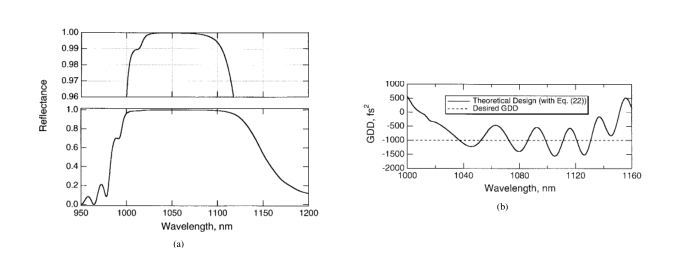
\includegraphics[width=\textwidth]{figures/anal.png}
    \caption[Współczynnik odbicia i GDD w przypadku rozwiązania analitycznego]{Współczynnik odbicia i GDD w przypadku rozwiązania analitycznego \cite{dbr3}}
    \label{fig:anal}
\end{figure}

Otrzymana wartość GDD jest niska, lecz nie jest do końca stabilna. Dlatego próbowano uzyskać jeszcze lepsze wartości tego parametru korzystając z innych podejść do problemu oraz z potęgi komputerów w celu zoptymalizowania obliczeń. W taki też sposób pojawiła się między innymi praca \cite{dbr2} wykorzystująca metodę macierzy przejścia, która jest szczegółowo omówiona w 3.1, w celu wyznaczenia wzorów pozwalających obliczyć współczynnik odbicia i GDD dla danego zwierciadła. Ponadto tę metodę zoptymalizowano korzystając z algorytmów genetycznych aby uzyskać jak najlepsze wyniki. Udało się wyznaczyć strukturę z wartością GDD wynoszącą około $-3600\fs$ przy zakresie długości fali $1030 - 1050\nm$. Metoda ta okazała się skuteczna, lecz wyniki wciąż można próbować polepszyć. Jedną z rzeczy, która jeszcze nie została zrobiona jest sprawdzenie efektu zastosowania innego rodzaju algorytmów, m.in. algorytmów rojowych, należących do grupy algorytmów stadnych.

Dlatego też niniejsza praca przedstawia próbę otrzymania jeszcze lepszych wyników wykorzystując optymalizację obliczeń przy wykorzystaniu algorytmów rojowych. Dodatkowym celem pracy było poznanie sposobu działania tych właśnie algorytmów i sprawdzenie ich potencjału przy rozwiązywaniu podobnych problemów.
%%2.	Teoria i istota zwierciadeł o niskiej dyspersji, przegląd literatury

\chapter{Przegląd literatury}
%\section{Metoda macierzy przejścia} \label{macierz} %3.	Opis metody macierzy przejścia 

Pierwszym etapem jest wyznaczenie funkcji pozwalającej na określenie wartości współczynnika odbicia R jak i GDD dla dowolnego zwierciadła DBR. Posłużymy się metodą macierzy przejścia, która polega na wyznaczeniu macierzy przejścia wektora natężenia pola elektrycznego z jednej warstwy do drugiej, a następnie, na tej podstawie, macierzy przejścia dla całej struktury.

Wiązka światłą padająca na zwierciadło DBR jest, zgodnie z istotą korpuskularno-falową światła, falą elektromagnetyczną. Pole elektryczne w każdej z warstw zwierciadła DBR ma postać:
\begin{equation}
    E_m(z) = F_me^{-in_m \frac\omega c z} + B_me^{in_m \frac\omega c z},
\end{equation}

gdzie $F_m$ i $B_m$ odpowiadają fali poruszającej się w kierunku $z$ z kolejno zwrotem dodatnim i ujemnym. \\
Pochodna powyższej wartości ma postać: 

\begin{equation}
    \frac{\partial E_m}{\partial z} = -i n_m \frac\omega c(F_me^{-in_m \frac\omega cz} - B_me^{in_m \frac\omega cz}).
\end{equation}

Na rysunku \ref{fig:transmatr} przedstawiono schemat ilustrujący rozkład sił pola elektrycznego w zwierciadle. Przyjmijmy $F'_m = F_m e^{-i\phi_m}$ i $B'_m = B_m e^{i\phi_m}$, gdzie $\phi = n_m \frac\omega c d_m$.
\begin{figure}[H]
    \centering
    \begin{tikzpicture}
        \draw (3,5) -- (3,0) 
        (1.5,5.3) node {$n_0$}
        (4,5.3) node {$n_1$}
        (3,-0.3) node {$z_0$};
        \draw (5,5) -- (5,0) 
        (6.5,5.3) node {$n_2$}
        (5,-0.3) node {$z_1$};
        \draw (8,5) -- (8,0) 
        (9,5.3) node {$n_3$}
        (8,-0.3) node {$z_2$};
        \draw (10,5) -- (10,0)
        (11.5,2.5) node {...}
        (10,-0.3) node {$z_3$};
        \draw (13,5) -- (13,0)
        (13,-0.3) node {$z_N$}
        (14,5.3) node {$n_N$};
        %skladowe F
        \draw[->] (2.25,3.5) -- (3,3.5) node[above left] {$F_0$};
        \draw[->] (3,3.5) -- (3.75,3.5) node[above] {$F_1$};
        \draw[color = red, ->] (4.25,3.5) -- (5,3.5) node[above left] {$F'_1$};
        \draw[->] (5,3.5) -- (5.75,3.5) node[above] {$F_2$};
        \draw[color = red, ->] (7.25,3.5) -- (8,3.5) node[above left] {$F'_2$};
        \draw[->] (8,3.5) -- (8.75,3.5) node[above] {$F_3$};
        \draw[color = red, ->] (9.25,3.5) -- (10,3.5) node[above left] {$F'_3$};
        \draw[->] (10,3.5) -- (10.75,3.5) node[above] {$F_4$};
        \draw[color = red, ->] (12.25,3.5) -- (13,3.5) node[above left] {$F'_{N-1}$};
        \draw[->] (13,3.5) -- (13.75,3.5) node[above] {$F_N$};
        %skladowe B
        \draw[<-] (2.25,1.5) -- (3,1.5) node[above left] {$B_0$};
        \draw[<-] (3,1.5) -- (3.75,1.5) node[above] {$B_1$};
        \draw[color = red, <-] (4.25,1.5) -- (5,1.5) node[above left] {$B'_1$};
        \draw[<-] (5,1.5) -- (5.75,1.5) node[above] {$B_2$};
        \draw[color = red, <-] (7.25,1.5) -- (8,1.5) node[above left] {$B'_2$};
        \draw[<-] (8,1.5) -- (8.75,1.5) node[above] {$B_3$};
        \draw[color = red, <-] (9.25,1.5) -- (10,1.5) node[above left] {$B'_3$};
        \draw[<-] (10,1.5) -- (10.75,1.5) node[above] {$B_4$};
        \draw[color = red, <-] (12.25,1.5) -- (13,1.5) node[above left] {$B'_{N-1}$};
        \draw[<-] (13,1.5) -- (13.75,1.5) node[above] {$B_{N}$};
    \end{tikzpicture}
    \caption{Schemat zwierciadła DBR}
    \label{fig:transmatr}
\end{figure}

Warunek ciągłości dla poszczególnych warstw można zapisać następująco:
\begin{equation}
    \left\{
    \begin{array}{l}
        F'_m + B'_m = F_{m+1} + B_{m+1}, \\
        n_m(F'_m - B'_m) = n_{m+1}(F_{m+1} - B_{m+1}).
    \end{array}
    \right.
\end{equation}
Rozwiązując powyższy układ równań względem $F'_m$ i $B'_m$ otrzymujemy:

\begin{equation}
    \left[
    \begin{array}{c}
    F_{m+1} \\ B_{m+1}
    \end{array}
    \right] = \frac 12
    \left[
    \begin{array}{cc}
         (1 + \frac{n_m}{n_{m+1}}) &  (1 - \frac{n_m}{n_{m+1}})\\
         (1 - \frac{n_m}{n_{m+1}}) &  (1 + \frac{n_m}{n_{m+1}})
    \end{array}
    \right]
    \left[
    \begin{array}{c}
    F'_{m} \\ B'_{m}
    \end{array}
    \right].
\end{equation}
Korzystając z definicji $F'_m$ i $B'_m$ możemy zapisać:
\begin{equation}
    \left[
    \begin{array}{c}
    F_{m+1} \\ B_{m+1}
    \end{array}
    \right] = \frac 12
    \left[
    \begin{array}{cc}
         (1 + \frac{n_m}{n_{m+1}}) &  (1 - \frac{n_m}{n_{m+1}})\\
         (1 - \frac{n_m}{n_{m+1}}) &  (1 + \frac{n_m}{n_{m+1}})
    \end{array}
    \right]
    \left[
    \begin{array}{c}
    e^{-i\phi_m} \\ e^{i\phi_m}
    \end{array}
    \right]
    \left[
    \begin{array}{c}
    F_{m} \\ B_{m}
    \end{array}
    \right],
\end{equation}
co ostatecznie daje:
\begin{equation}
    \left[
    \begin{array}{c}
    F_{m+1} \\ B_{m+1}
    \end{array}
    \right] = \frac 12
    \left[
    \begin{array}{cc}
         (1 + \frac{n_m}{n_{m+1}})e^{-i\phi_m} &  (1 - \frac{n_m}{n_{m+1}})e^{i\phi_m}\\
         (1 - \frac{n_m}{n_{m+1}})e^{-i\phi_m} &  (1 + \frac{n_m}{n_{m+1}})e^{i\phi_m}
    \end{array}
    \right]
    \left[
    \begin{array}{c}
    F_{m} \\ B_{m}
    \end{array}
    \right].
\end{equation}
Macierz $    \left[
    \begin{array}{cc}
         (1 + \frac{n_m}{n_{m+1}})e^{-i\phi_m} &  (1 - \frac{n_m}{n_{m+1}})e^{i\phi_m}\\
         (1 - \frac{n_m}{n_{m+1}})e^{-i\phi_m} &  (1 + \frac{n_m}{n_{m+1}})e^{i\phi_m}
    \end{array}
    \right]$ nazywamy macierzą przejścia i notujemy $T_m$.
    
Dla lepszej czytelności zapiszmy $E_m =     \left[
    \begin{array}{c}
    F_{m} \\ B_{m}
    \end{array}
    \right]$.
Można zauważyć, że wartość natężenia pola elektrycznego dla danej warstwy zależy od wartości natężenia dla warstwy poprzedniej:
    
\begin{align*}
    &E_1 = T_0 E_0, \\
    &E_2 = T_1 T_0 E_0, \\
    &... \\
    &E_N = (T_N ... T_1 T_0) E_0.
\end{align*}

Iloczyn poszczególnych macierzy przejścia, tj. macierz $T = T_N ... T_1 T_0$, nazywamy macierzą przejścia całej struktury.
Zapiszmy macierz przejścia całej struktury w sposób następujący:
$T = \left[
\begin{array}{cc}
   t_1  & t_2 \\
   t_3  & t_4
\end{array}
\right]$.

Korzystając z tak obliczonej macierzy przejścia można obliczyć amplitudowy współczynnik odbicia, który definiuje stosunek amplitudy fali odbitej do fali padającej. Jako, że $t_3$ odpowiada fali odbitej, natomiast $t_4$ fali padającej, można otrzymać wzór $r=-\frac{t_3}{t_4}$,
%Amplitudowy współczynnik transmisji $t = t_1 - \frac{t_2t_3}{t_4}$
oraz, na tej podstawie, współczynnik odbicia $R = rr^*$.
%Współczynnik transmisji $T = \frac{n_N}{n_0}tt^*$

Grupowe opóźnienie GD (Group Delay) można zdefiniować jako pierwsza pochodna zmiany fazy $\phi$ po częstotliwości $\omega$. Wiemy, że zmianę fazy można zapisać w postaci:
\begin{equation}
    \phi = \arctan\left(\frac{\mathrm{Im}(r)}{\mathrm{Re}(r)}\right),
\end{equation}
stąd GD obliczamy korzystając ze wzoru:

\begin{equation}
    GD = \frac{d\phi}{d\omega} = \frac{\mathrm{Im}(r) \frac{d}{d\omega}\mathrm{Re}(r) - \mathrm{Re}(r) \frac{d}{d\omega}\mathrm{Im}(r)}{rr^*} ,
\end{equation}
natomiast GDD jest pochodną GD po częstotliwości $\omega$, tak jak to przedstawiono we wzorze poniżej:

\begin{equation}
    GDD = \frac{d}{d\omega} GD.
\end{equation}

Tak otrzymane wzory posłużyły do sporządzenia modelu zwierciadła DBR (w postaci klasy) umożliwiającego obliczenie GDD i R dla danego zwierciadła. %Aby dokonać obliczeń wystarczy stworzyć nowy obiekt klasy \textit{DBRMirror} podając dane w postaci współczynników załamania i grubości dla poszczególnych warstw zwierciadła. Stworzenie takiego obiektu skutkuje automatycznym dokonaniem obliczeń i od tego momentu wartości GDD i R są dostępne jako atrybuty tej klasy.
%4.	Opis algorytmu rojowego (rozróżnić co z literatury co sam wymyśliłem)
%a.	Test dla zwykłej funkcji

\chapter{Algorytmy rojowe} \label{algo}

Po ogólnym wprowadzeniu do tematu w rozdziale \ref{wstep}, czas przejść do omówienia zastosowanej metody. Jednym z bardziej rzucających się w oczy wyrażeń w tytule pracy jest "algorytmy rojowe" i to właśnie nimi zajmiemy się w tym rozdziale. Zostanie omówiona istota algorytmów rojowych, zarówno w literaturze jak i ostateczna wersja zastosowana w programie, oraz, na koniec, zostanie przedstawiony przykład implementacji na funkcji dwóch zmiennych.

%----------------------------------------------------------------------------------------
%----------------------------------------------------------------------------------------
%----------------------------------------------------------------------------------------

\section{Algorytmy rojowe w literaturze}

Algorytmy rojowe należą do rodziny algorytmów stadnych. Ich główną ideą jest wykorzystanie sposobu zachowywania się pszczół zwiadowców podczas zbierania nektaru. Pszczoły, zgodnie z \cite{algroj}, wyruszają na łąkę w poszukiwaniu kwiatów z dużą ilością nektaru. Następnie wracają do ula i wykonują tak zwany taniec pszczeli podczas którego dochodzi do wymiany informacji między pszczołami na temat lokalizacji kwiatów o dużej zawartości nektaru. To pozwala na wysłanie pozostałych pszczół (czyli tych, które nie znalazły dobrych źródeł nektaru) do najlepszych lokalizacji. Im źródło zawiera więcej nektaru, tym więcej pszczół kieruje się do niego.

W literaturze (\cite{algroj}, \cite{algroj2}, \cite{algroj3}) można znaleźć różne opisy funkcjonowania tych algorytmów. Podejście różni się od źródła do źródła, lecz ogólny przebieg algorytmu rojowego jest taki sam i przedstawia się następująco:
\newpage
\begin{enumerate}
    \setcounter{enumi}{-1}
    \item inicjalizacja parametrów przekazanych programowi przy uruchomieniu:
     \begin{itemize}
        \item[$w_{best}$] - współczynnik określający procent rozwiązań uważanych za najlepsze względem wszystkich rozwiązań,
        \item[$w_{qual}$] - współczynnik określający procent rozwiązań uważanych za dobre względem wszystkich rozwiązań,
        \item[$w_{better}$] - współczynnik określający w jaki sposób pszczoły podzielą się na rozwiązania dobre i najlepsze. Jest to wartość z zakresu $(0, 1)$ i im jest większa tym więcej pszczół zostanie przydzielonych do przeszukiwania obszaru wokół rozwiązań najlepszych,
        \item[$d_{near}$] - wartość określająca odległość przeszukiwania od rozwiązania pierwotnego (sąsiedztwo),
        \item[$N$] - liczba pszczół zwiadowców biorąca udział w poszukiwaniu rozwiązania,
    \end{itemize}
     oraz zmiennych:
    \begin{itemize}
        \item[$n$] - liczba wszystkich rozwiązań,
        \item[$n_{best}$] - liczba najlepszych rozwiązań (w chwili początkowej$ = 0$) określona współczynnikiem $w_{best}$,
        \item[$n_{qual}$] - liczba rozwiązań dobrych (w chwili początkowej$ = 0)$ określona współczynnikiem $w_{qual}$,
        \item[$n_{left}$] - liczba rozwiązań pozostałych (nie zdefiniowanych jako dobre lub najlepsze) (w chwili początkowej$ = 0$),
    \end{itemize}
   \label{e1}
   \item wygenerowanie początkowych $N$ rozwiązań,
    \item ocena znalezionych rozwiązań przy użyciu funkcji celu, podział ich na kategorie (najlepsze, dobre i pozostałe lub dobre i pozostałe), \label{e2}
    \item przeszukiwanie sąsiedztwa najlepszych znalezionych rozwiązań w promieniu $d_{near}$ od danego rozwiązania, \label{e3}
     \item wybranie najlepszego rozwiązania z każdej przeszukiwanej lokalizacji, \label{e4}
    \item zapisanie najlepszego rozwiązania, \label{e5}
    \item generacja nowej populacji rozwiązań w zadanym obszarze, uwzględniając te znalezione w etapie \ref{e3}, tak aby ich liczba osiągnęła $N$, \label{e6} 
    \item powrót do etapu \ref{e2} lub zakończenie działania programu w przypadku spełnienia warunku stopu.\label{e7}
\end{enumerate}

W celu lepszego zilustrowanie działania algorytmu zostały wykonane schematy na rysunku \ref{fig:schemat_roj}. Przebieg przedstawiony tam odpowiada dokładnie temu opisanemu w \cite{algroj}.

\begin{figure} [htbp]
    \centering
    \begin{subfigure}[b]{0.32\textwidth}
    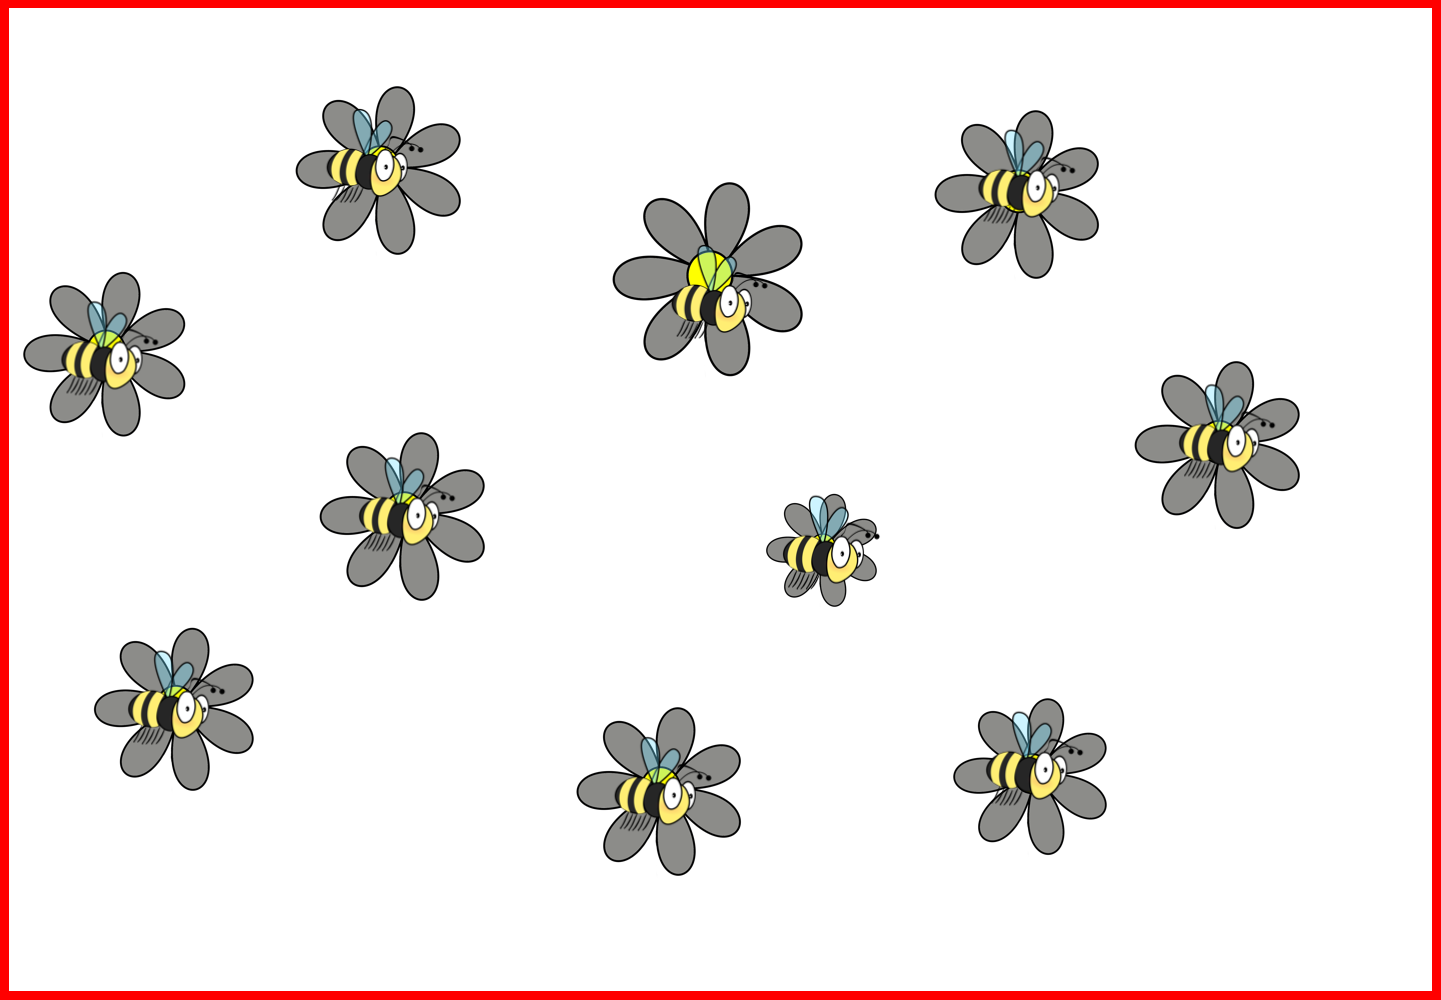
\includegraphics[width=\linewidth]{figures/rojowe/etap2.png}
    \caption{Losowanie rozwiązań\\~\\~\\~}
    \end{subfigure}
    \begin{subfigure}[b]{0.32\textwidth}
    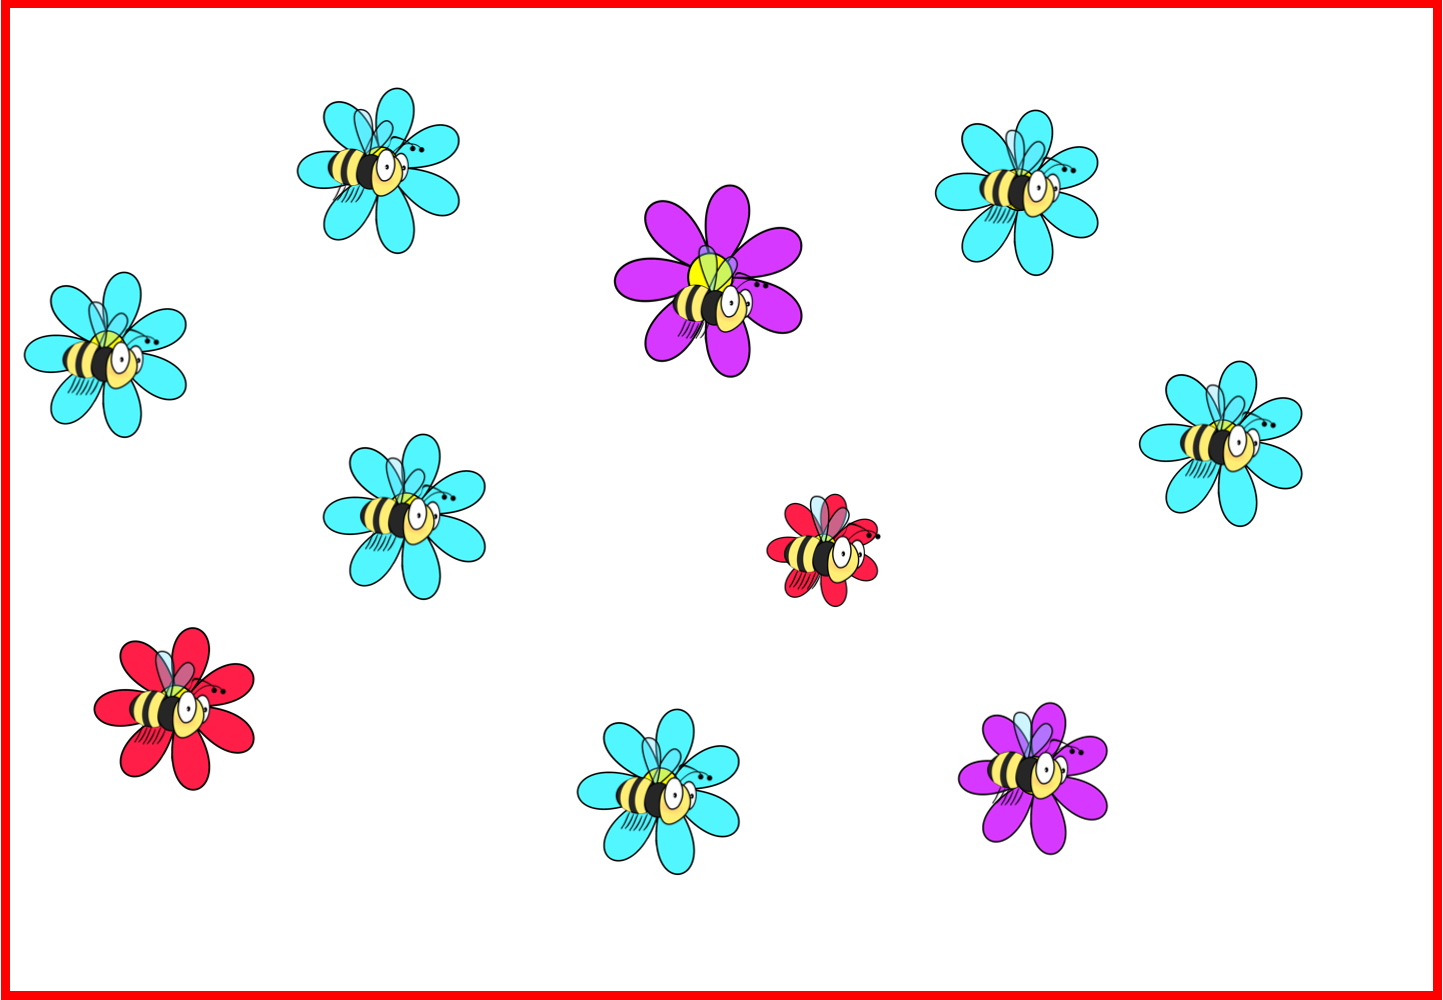
\includegraphics[width=\linewidth]{figures/rojowe/etap3.png}
    \caption{Ocena rozwiązań\\~\\~\\~}
    \end{subfigure}
    \begin{subfigure}[b]{0.32\textwidth}
    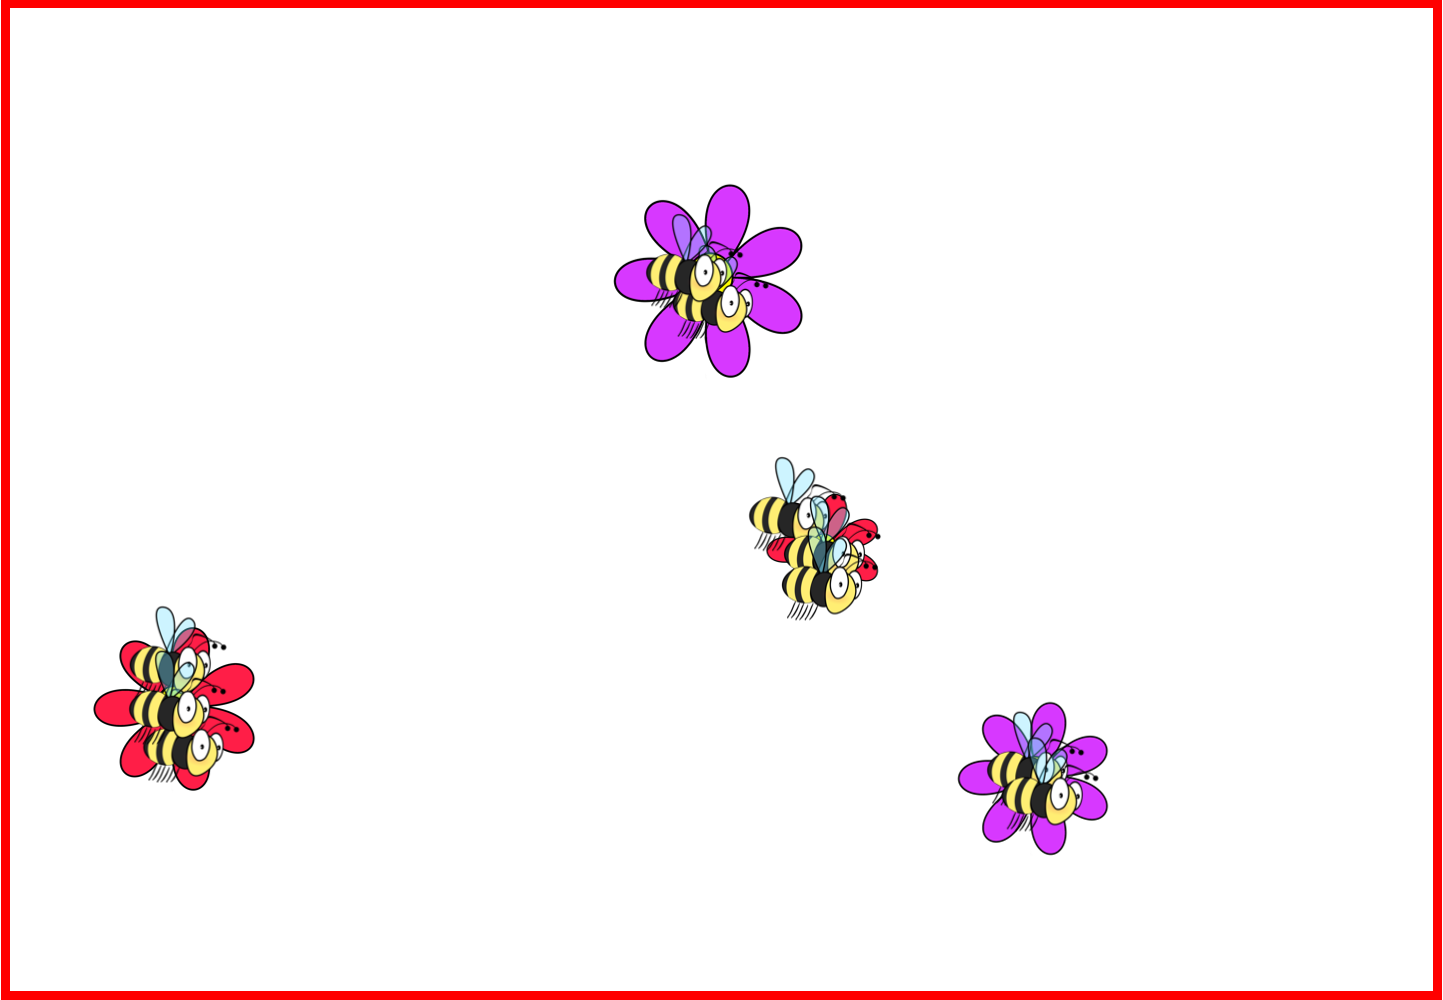
\includegraphics[width=\linewidth]{figures/rojowe/etap4.png}
    \caption{Przydział pszczół do rozwiązań dobrych i najlepszych oraz porzucenie pozostałych rozwiązań}
    \end{subfigure}
    \begin{subfigure}[b]{0.32\textwidth}
    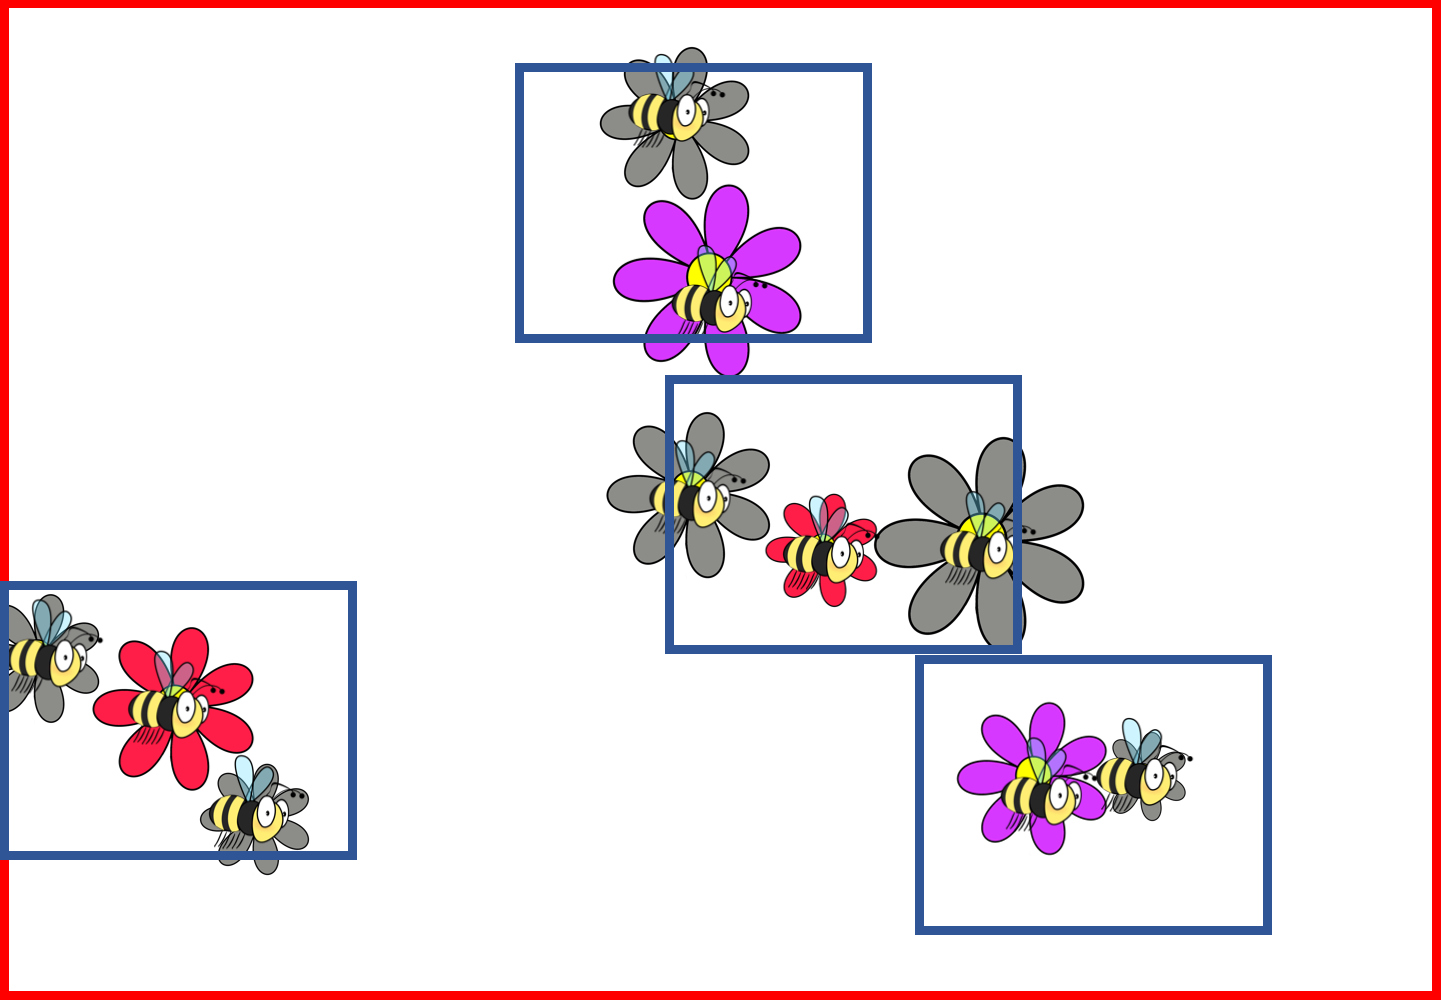
\includegraphics[width=\linewidth]{figures/rojowe/etap5.png}
    \caption{Losowanie rozwiązań w sąsiedztwie rozwiązań, które pozostały}
    \end{subfigure}
    \begin{subfigure}[b]{0.32\textwidth}
    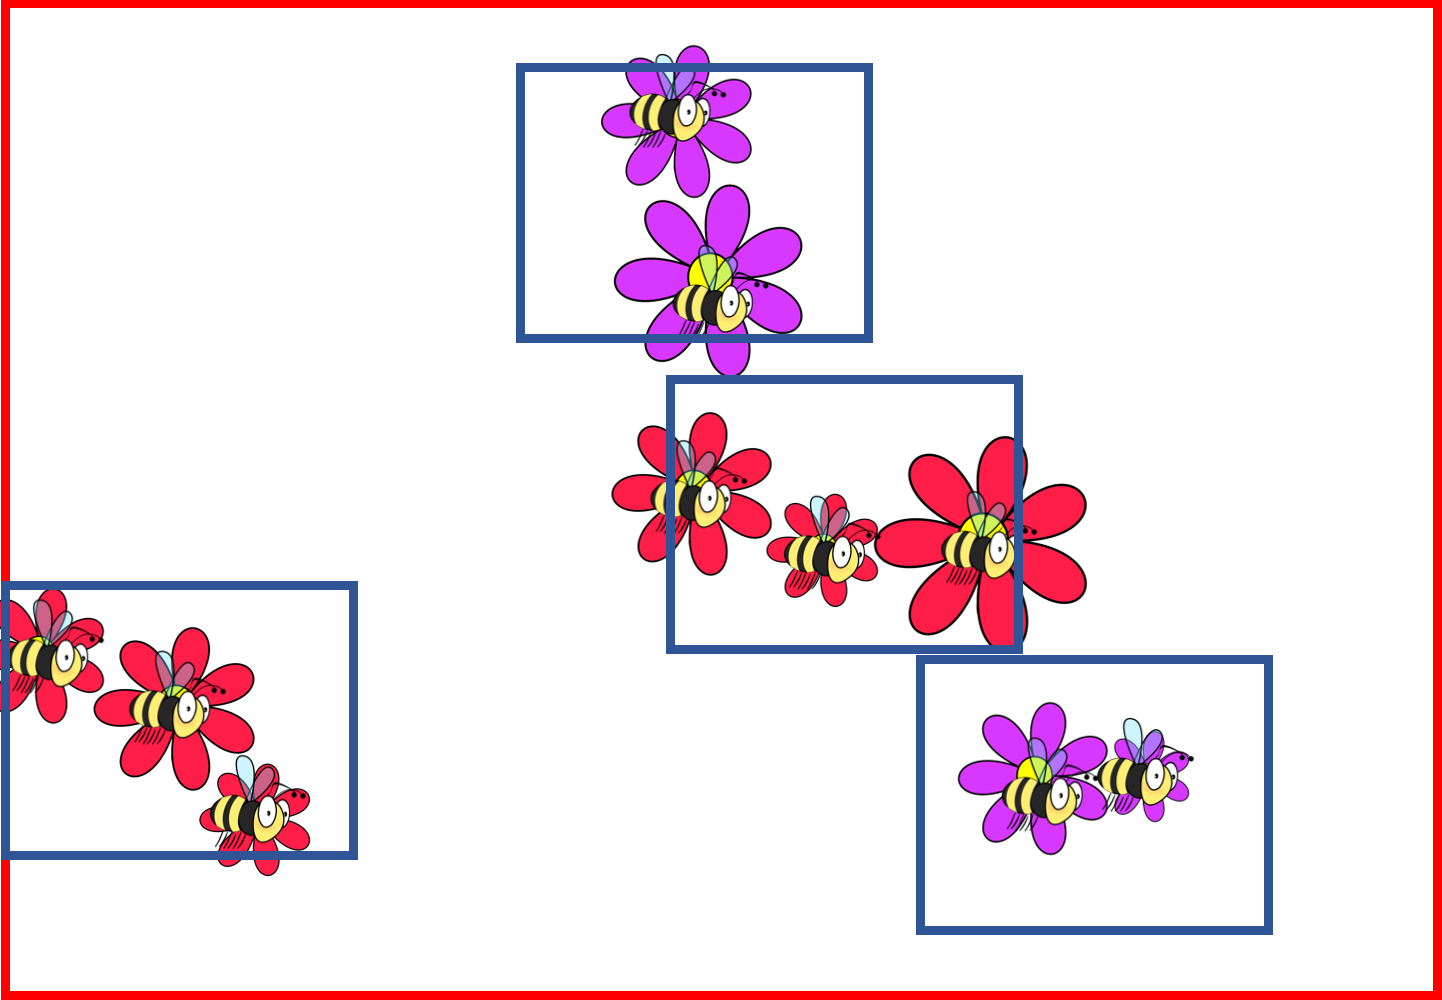
\includegraphics[width=\linewidth]{figures/rojowe/etap6.png}
    \caption{Ocena rozwiązań z sąsiedztwa\\~}
    \end{subfigure}
    \begin{subfigure}[b]{0.32\textwidth}
    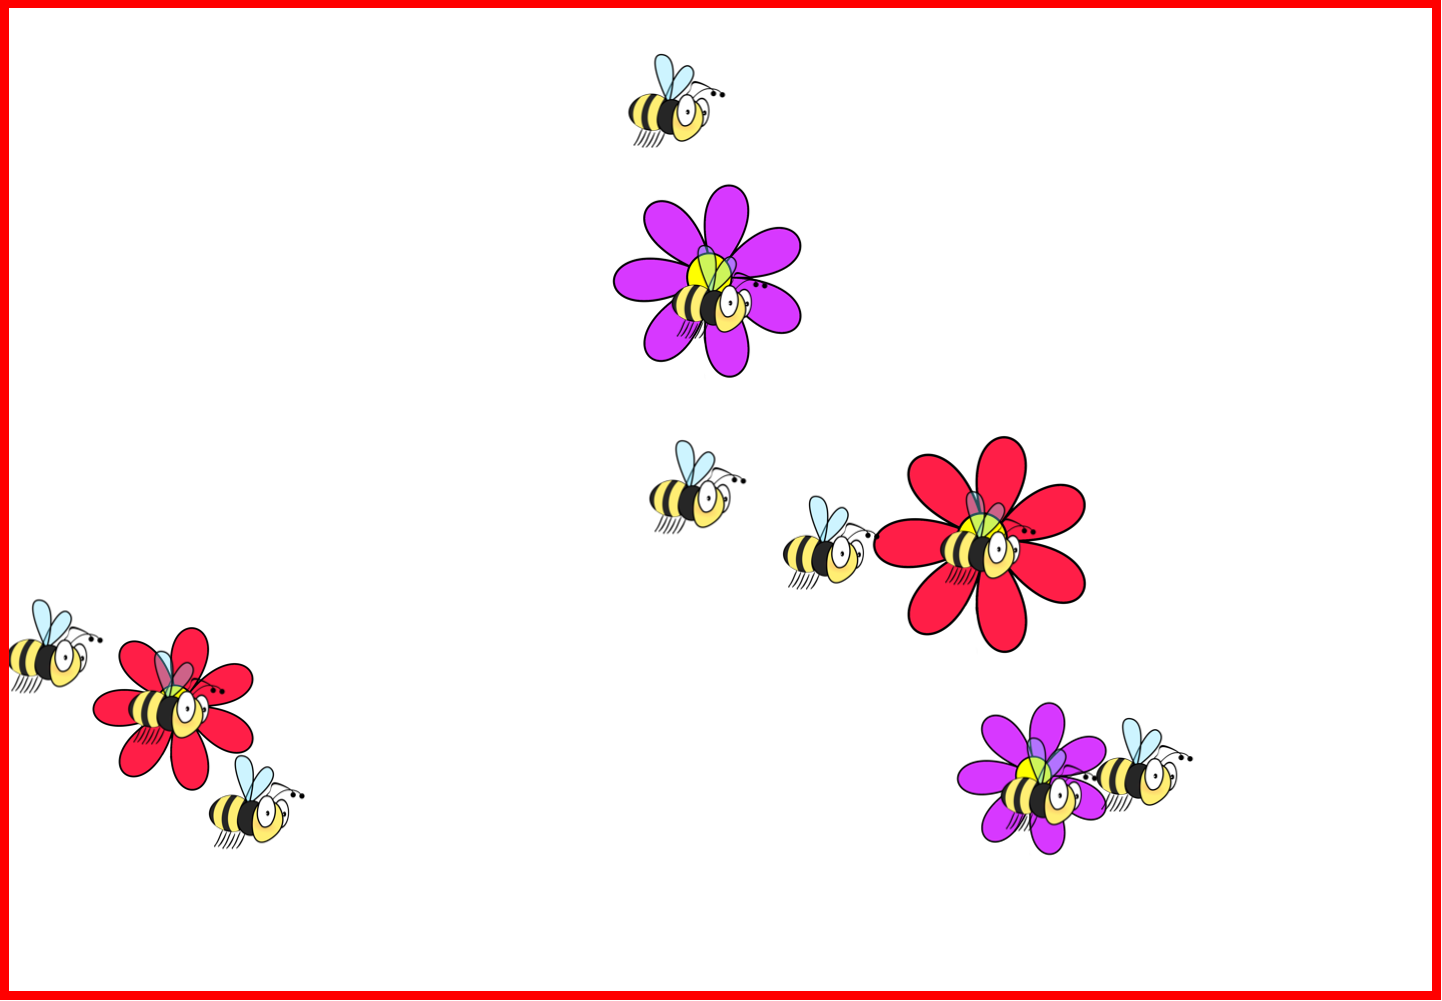
\includegraphics[width=\linewidth]{figures/rojowe/etap7.png}
    \caption{Wybór najlepszego rozwiązania z każdego obszaru}
    \end{subfigure}
    \begin{subfigure}[b]{0.32\textwidth}
    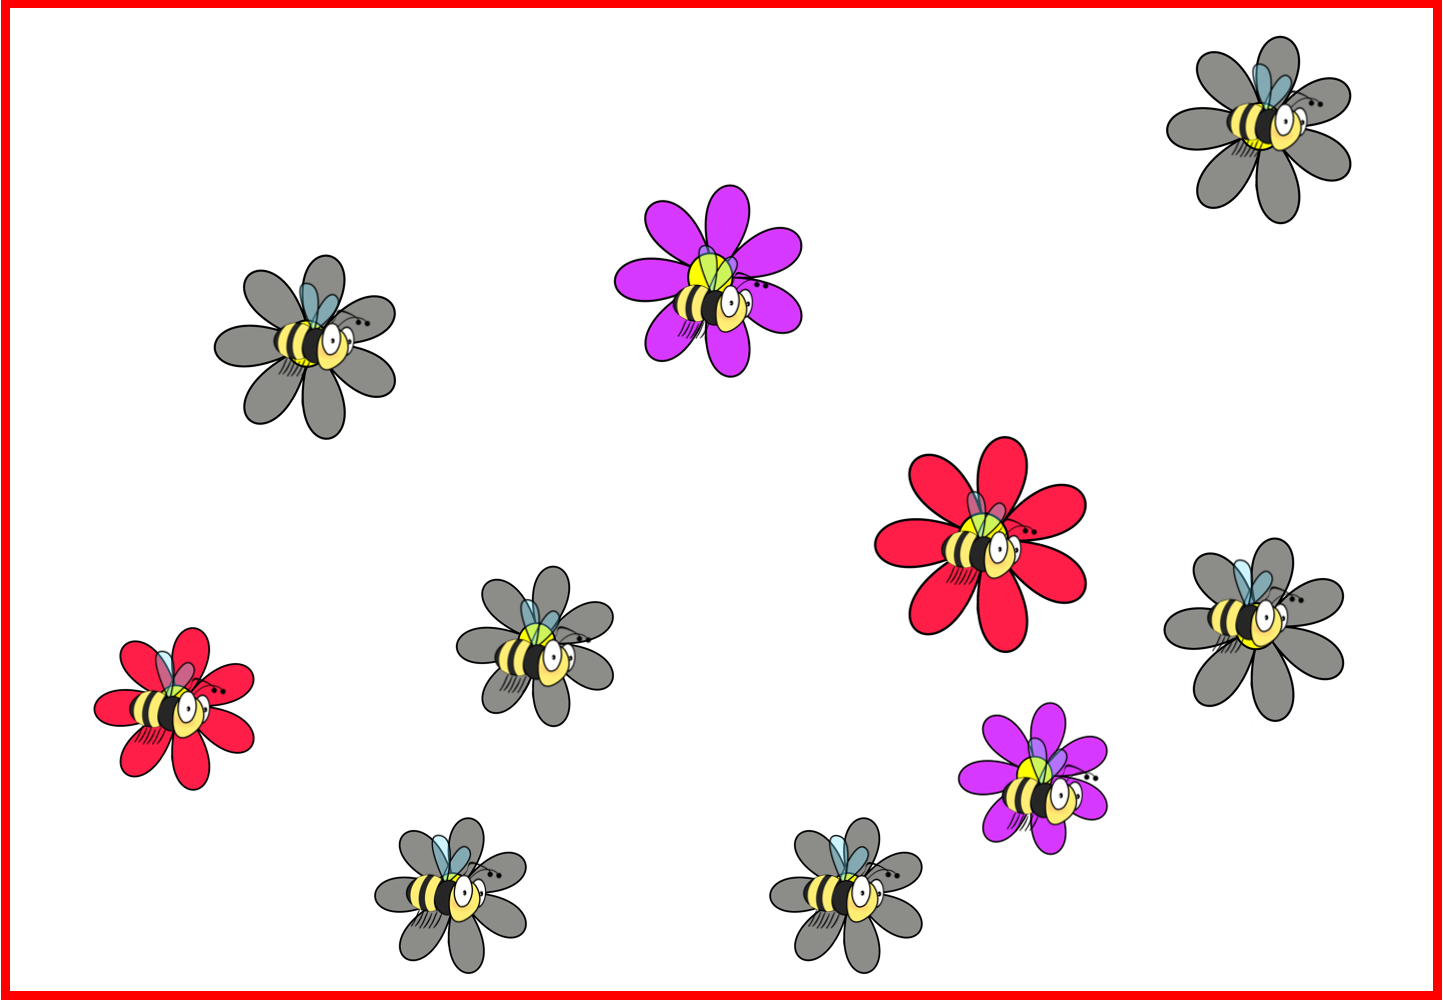
\includegraphics[width=\linewidth]{figures/rojowe/etap8.png}
    \caption{Pszczoły, które nie znalazły najlepszych rozwiązań, zostają przydzielone do nowych losowych rozwiązań}
    \end{subfigure}
    \begin{subfigure}[b]{0.32\textwidth}
    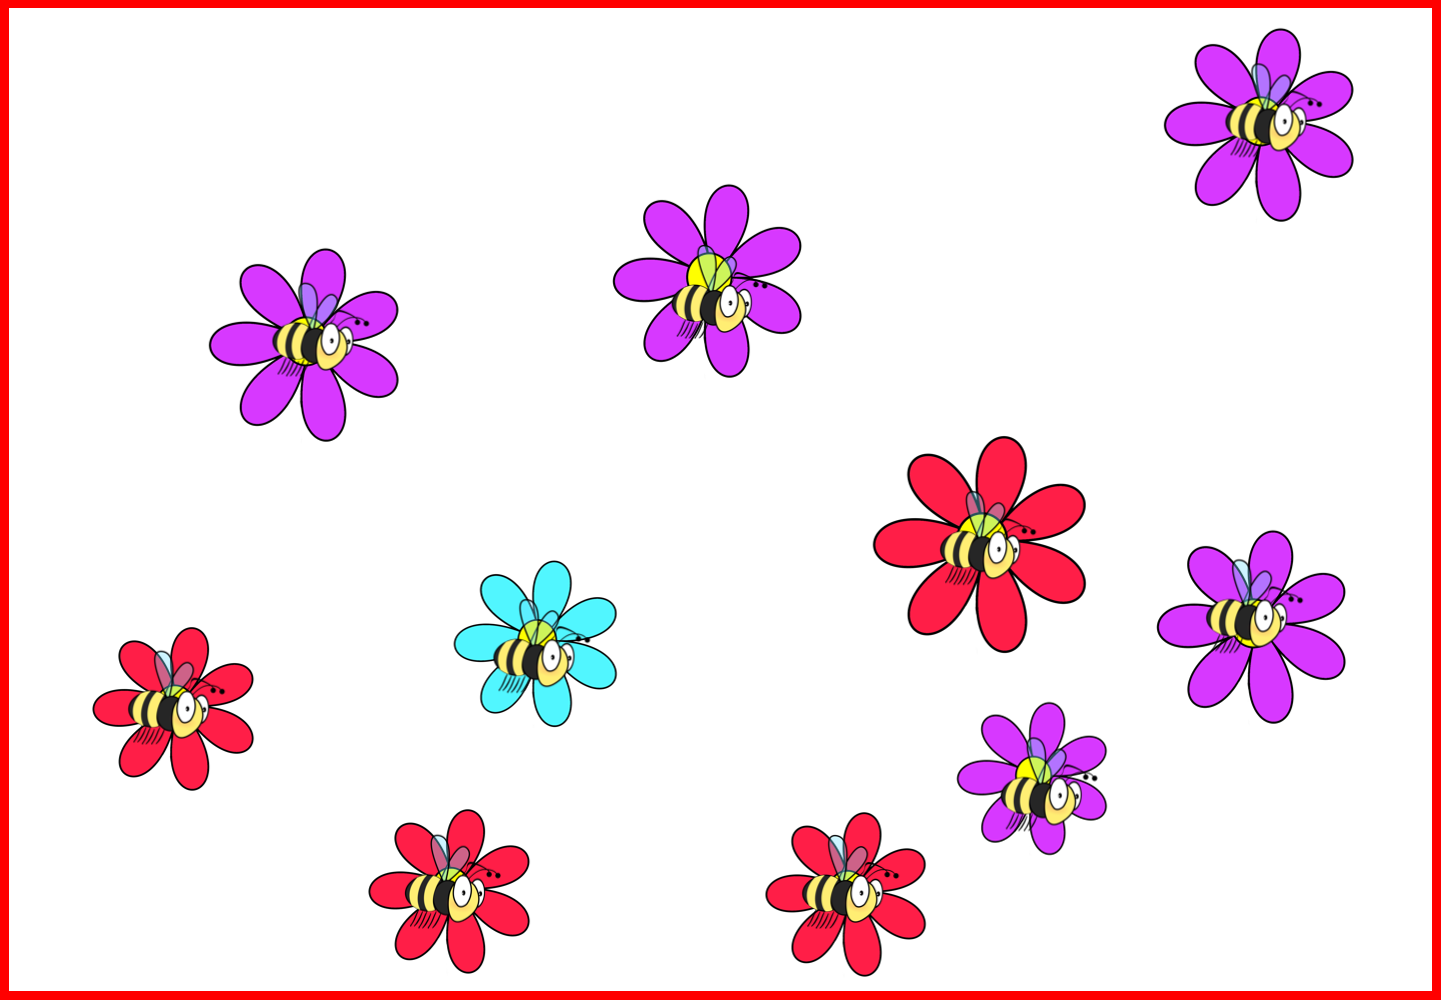
\includegraphics[width=\linewidth]{figures/rojowe/etap9.png}
    \caption{Ocena tak znalezionych rozwiązań\\~\\~\\~}
    \end{subfigure}
    \caption[Ilustrowany schemat działania algorytmu rojowego]{Ilustrowany schemat działania algorytmu rojowego zgodnie z \cite{algroj}.} 
    Oznaczenia: kwiatek czerwony --- rozwiązanie najlepsze, kwiatek fioletowy --- rozwiązanie dobre, kwiatek błękitny --- rozwiązanie z grupy pozostałych, czerwony prostokąt --- obszar losowania rozwiązań, niebieski prostokąt --- obszar sąsiedztwa danego rozwiązania, rozmiar kwiatka świadczy o jakości rozwiązania w swojej kategorii, tj. im kwiatek większy tym rozwiązanie lepsze.
    \label{fig:schemat_roj}
\end{figure}

Wszelkie różnice pojawiają się w szczegółowym przebiegu poszczególnych etapów. Pierwsza taka zauważalna różnica pojawia się w etapie \ref{e2}, gdzie niektóre źródła (\cite{algroj} i \cite{algroj3}) proponują podział ocenionych rozwiązań na dobre i najlepsze na podstawie parametrów $w_{best}$ i $w_{qual}$. W \cite{algroj} te parametry oznaczają wartość funkcji celu od jakiej dane rozwiązanie jest rozumiane jako dobre lub elitarne, natomiast w \cite{algroj3} są to parametry które określają procent rozwiązań z danej kategorii względem wszystkich rozwiązań. Inne źródła (\cite{algroj2}) proponują posortowanie rozwiązań od najlepszego do najgorszego bez rozróżniania najlepszych i elitarnych. Następnie, w etapie \ref{e3}, przy przeszukiwaniu rozwiązań, w \cite{algroj} i \cite{algroj3} przydziela się odpowiednią ilość pszczół zwiadowców do przeszukania sąsiedztwa danego rozwiązania w zależności od rangi rozwiązania (elitarne bądź dobre) zgodnie z parametrem $w_{better}$. Ten parametr ilustruje stosunek ilości pszczół przypisanych do przeszukiwania sąsiedztwa rozwiązań dobrych i elitarnych. Natomiast w \cite{algroj2}, biorąc pod uwagę brak podziału na dobre i elitarne, pszczoły są przydzielane w równych proporcjach do rozwiązań, które zostały wyznaczone do przeszukania ich sąsiedztwa. Ponadto, etap \ref{e5} jest pominięty w \cite{algroj}, ale nie odgrywa on szczególnie ważnej roli, gdyż najlepszy wynik zawsze przechodzi do następnej iteracji i zawsze istnieje możliwość jego odczytania.

Z dodatkowych różnic można wspomnieć wprowadzenie długości życia rozwiązania w \cite{algroj3}. Ta długość życia miałaby pozwolić na wyeliminowanie rozwiązań, które będą się powtarzać przez określoną wcześniej liczbę iteracji.  

%----------------------------------------------------------------------------------------
%----------------------------------------------------------------------------------------
%----------------------------------------------------------------------------------------

\section{Algorytm zastosowany w programie}

Algorytm zastosowany w tejże pracy przeszedł parę delikatnych transformacji przez cały czas sporządzania finalnego modelu wartości dyspersyjnych zwierciadła DBR. Jako algorytm wejściowy został zastosowany ten opisany w \cite{algroj}. Na początku funkcja celu została zaprojektowana tak, aby zwracała wartości z zakresu (0,1). Rozwiązania elitarne i dobre były ustalane na podstawie porównania wartości zwróconej przez funkcję celu z dwoma parametrami algorytmu, określającymi próg, od którego rozwiązania jest uznawane za dobre i próg, od którego rozwiązanie jest uznawane za elitarne. Dla tak dobranych rozwiązań, w sposób losowy, były generowane rozwiązania z sąsiedztwa danego rozwiązania. Po etapie \ref{e5} polegającym na zapisaniu najlepszego rozwiązania, algorytm sprawdzał czy suma rozwiązań dobrych i elitarnych nie przekroczyła danego progu będącego parametrem algorytmu, jeśli tak, wówczas próg minimalnej wartości funkcji celu dla rozwiązań dobrych i elitarnych był zwiększany oraz rozmiar sąsiedztwa rozwiązań był zwężany. Dodanie tego etapu wynikało z chęci przyspieszenia dążenia algorytmu do rozwiązania i nie występuje on w żadnym z wymienionych źródeł.

Po wielu testach zauważono, iż algorytm napotyka problemy przy generowaniu rozwiązań spełniających próg rozwiązań dobrych i elitarnych. Większość rozwiązań otrzymywała ocenę równą zeru. Problem polegał na funkcji celu i trudności w otrzymaniu oceny umożliwiającej rozróżnienie jakości wszystkich wygenerowanych rozwiązań, przy zachowaniu skali oceny w zakresie (0,1). Ten fakt wynikał z tego, iż cel, który program miałby osiągnąć nie mógł zostać określony w sposób jednoznaczny, aby móc ustalić maksymalną wartość rozwiązań jakie zostaną wygenerowane. Dlatego też funkcja celu została zmodyfikowana w taki sposób aby wystawiać ocenę rozwiązania bez korzystania z jakiejkolwiek skali. Tak zbudowana funkcja celu jest w stanie rozróżnić między jakością każdego wygenerowanego rozwiązania, lecz bez możliwości jednoznacznego określenia maksymalnej i minimalnej oceny jaką może wystawić. Ten fakt spowodował konieczność modyfikacji algorytmu. Zamiast wyznaczania rozwiązań elitarnych i dobrych na podstawie progów, rozwiązania są teraz sortowane na podstawie wartości funkcji celu od najlepszego do najgorszego, tak jak w \cite{algroj3}. Następnie, na podstawie parametrów $w_{best}$ i $w_{qual}$ określającymi procent rozwiązań elitarnych i dobrych względem wszystkich rozwiązań, rozwiązania są kategoryzowane. Dla przykładu, jeżeli bierzemy pod uwagę $100$ rozwiązań i parametry $w_{best}$ i $w_{qual}$ wynoszą kolejno $0,1$ i $0,2$, po posortowaniu od najlepszego do najgorszego pierwsze 10 rozwiązań jest uznawane za najlepsze, natomiast 20 następnych rozwiązań jako dobre. Dalej przebieg wygląda tak samo jak w źródle \cite{algroj}.

W algorytmie dodatkowo dopuszczono generowanie rozwiązań początkowych w odległości $d_{far}$ od rozwiązania początkowego załadowanego z zewnątrz programu. Warto zauważyć, że $d_{far}$ jest dużo większe od $d_{near}$.

Finalny algorytm zastosowany w programie został zaprezentowany na rysunku \ref{fig:algorytm_koncowy}.

\begin{figure}[H]
    \centering
    \begin{tikzpicture}[node distance=2.5cm]
    \node (gen) [bullet] {Wygenerowanie $n$ rozwiązań};
    \node (ocen) [bullet, below of=gen] {Ocena wygenerowanych rozwiązań i ich posortowanie};
    \node (best) [bullet, below of=ocen, xshift=-100] {Przypisanie $n_{best} = w_{best}\cdot n$ pierwszych najlepszych rozwiązań do rozwiązań elitarnych};
    \node (qual) [bullet, below of=ocen,xshift=100] {Przypisanie $n_{qual} = w_{qual}\cdot n$ następnych najlepszych rozwiązań do rozwiązań dobrych};
    \node (beese) [bullet, below of=best] {Przypisanie $n_{best} = n_{best} + w_{better}\cdot n_{left}$ pszczół do przeszukiwania sąsiedztwa rozwiązań elitarnych};
    \node (beesm) [bullet, below of=qual] {Przypisanie $n_{qual} = n_{qual} + (1-w_{better})\cdot n_{left}$ pszczół do przeszukiwania sąsiedztwa rozwiązań dobrych};
    \node (ocena) [bullet, below of=beese,xshift=100] {Ocena znalezionych rozwiązań};
    \node (wybor) [bullet, below of=ocena] {Wybór jednego rozwiązania z każdej przeszukiwanej lokalizacji};
    \node (najlepszy) [bullet, below of=wybor] {Wybór najlepszego znalezionego rozwiązania};
    \node (cel) [bullet, below of=najlepszy,fill=yellow!30] {Czy warunek stopu spełniony?};
    \node (koniec) [bullet, below of=cel] {Koniec działania algorytmu. Zapis podsumowania do pliku};
    \node (konty) [bullet, below of=najlepszy,xshift=200, text width=0.2\linewidth] {Wygenerowanie $n-n_{best}-n_{qual}$ losowych rozwiązań};
    \draw [arrow] (konty) |- (ocen);
    \draw [arrow] (gen) -- (ocen);
    \draw [arrow] (ocen) -- (best);
    \draw [arrow] (ocen) -- (qual);
    \draw [arrow] (best) -- (beese);
    \draw [arrow] (qual) -- (beesm);
    \draw [arrow] (beese) -- (ocena);
    \draw [arrow] (beesm) -- (ocena);
    \draw [arrow] (ocena) -- (wybor);
    \draw [arrow] (wybor) -- (najlepszy);
    \draw [arrow] (najlepszy) -- (cel);
    \draw [arrow,, color=black!60!green] (cel) -- node[anchor=east, color=black!60!green] {TAK} (koniec);
    \draw [arrow, color=black!40!red] (cel) -- node[anchor=south, color=black!40!red] {NIE} (konty);
    \end{tikzpicture}
    \caption{Przebieg algorytmu rojowego zastosowanego w programie}
    \label{fig:algorytm_koncowy}
\end{figure}

%----------------------------------------------------------------------------------------
%----------------------------------------------------------------------------------------
%----------------------------------------------------------------------------------------

\section{Przykład zastosowania na funkcji prostej}
W celu sprawdzenia efektywności algorytmu zostały wykonane testy na prostej funkcji dwóch zmiennych. Została wybrana funkcja Ackleya o wzorze:
\begin{equation}
f(x,y) = -20\exp\left[-0.2\sqrt{0.5\left(x^{2}+y^{2}\right)}\right] -\exp\left[0.5\left(\cos 2\pi x + \cos 2\pi y \right)\right] + e + 20,
\end{equation}

ze względu na to iż charakteryzuje się falistym wykresem z dużą ilością minimów lokalnych o wartościach malejących przy oddalaniu się od punktu $(0, 0)$, w którym to też znajduje się minimum globalne funkcji o wartości 0. Dla lepszego zobrazowania tej charakterystycznej struktury, wykres funkcji Ackleya został zaprezentowany na rysunku \ref{fig:ackley}.

\begin{figure}[H]
    \centering
    \begin{tabular}{cc}
         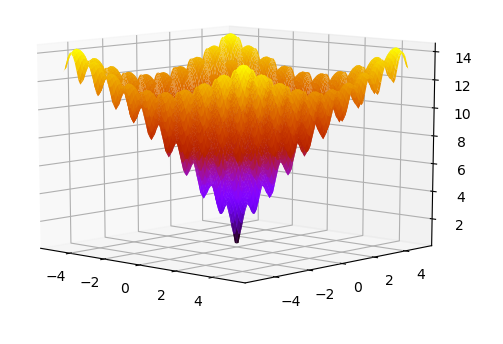
\includegraphics[width=0.5\linewidth]{figures/ackley1.png}& 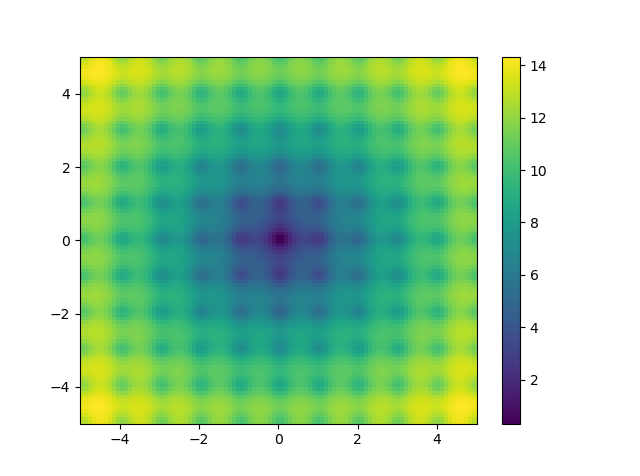
\includegraphics[width=0.5\linewidth]{figures/ackley2.png}
    \end{tabular}
    \caption{Funkcja Ackleya}
    \label{fig:ackley}
\end{figure}

Oprócz doboru badanej funkcji, bardzo istotnym elementem było określenie funkcji celu. W tym wypadku funkcja celu została zaprogramowana tak, że zwraca wartości z przedziału $\langle 0, 1 \rangle$ na podstawie modułu różnicy wartości funkcji od wartości $0$ w punkcie $(0, 0)$. Otrzymana liczba jest dzielona przez największą wartość jaką może przyjąć funckja w danych przedziale (w tej symulacji dla x i y w przedziale $\langle -1,5, 1,5\rangle$ maksymalna wartość funkcji wynosi $8$) i tak otrzymana liczba jest odejmowana od $1$ aby otrzymać skalę ocen w taki sposób, że im punkt bliższy rozwiązaniu tym ocena wyższa.

Symulacja została wykonana dla $N=1000$ zwiadowców, przy następujących wartościach parametrów: $d_{near} = 0,0005$, $w_{qual} = 0,20$, $w_{best} = 0,10$, $w_{better} = 0,6$. Wyniki obliczeń zostały przedstawione w tabeli \ref{tab:wyniki3d}.

\begin{table}[H]
    \centering
    \caption{Wyniki dla funkcji Ackleya}
    \begin{tabular}{cc}
         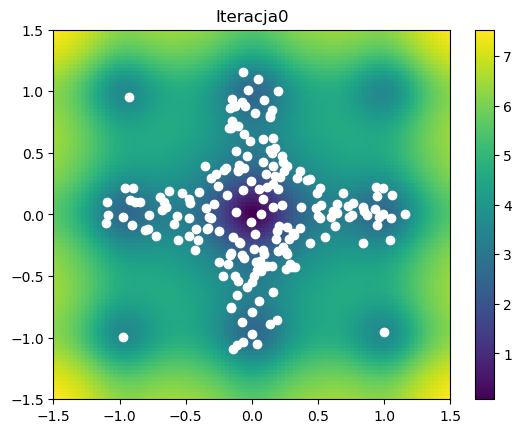
\includegraphics[width=0.5\linewidth]{figures/3d/it0.png} & 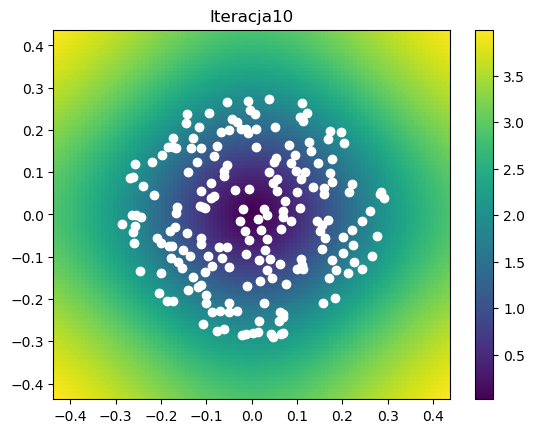
\includegraphics[width=0.5\linewidth]{figures/3d/it10.png} \\
         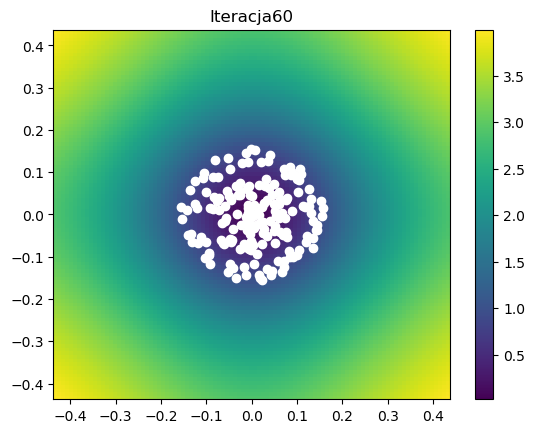
\includegraphics[width=0.5\linewidth]{figures/3d/it60.png} & 
         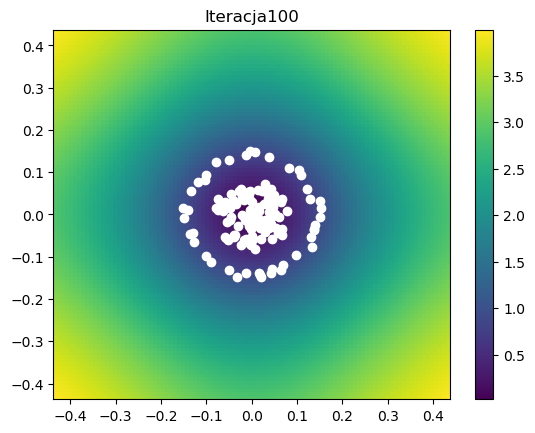
\includegraphics[width=0.5\linewidth]{figures/3d/it100.png} \\
         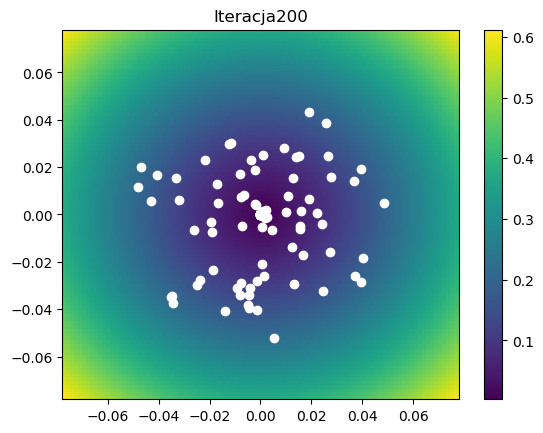
\includegraphics[width=0.5\linewidth]{figures/3d/it200.png} &
         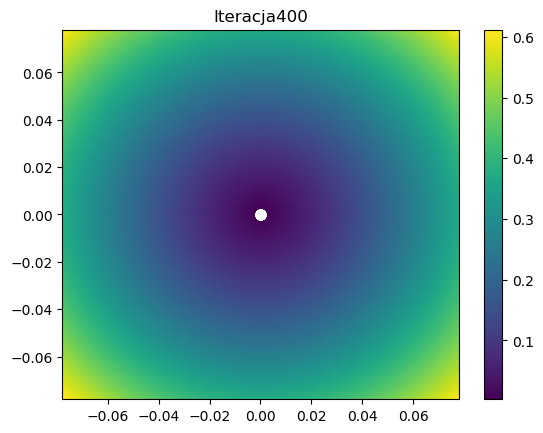
\includegraphics[width=0.5\linewidth]{figures/3d/it400.png}
    \end{tabular}
    \label{tab:wyniki3d}
\end{table}

Można zauważyć na podstawie wyników z tabeli \ref{tab:wyniki3d}, że z iteracji na iterację obszar poszukiwań zawęża się do coraz to bliższego sąsiedztwa poszukiwanego rozwiązania, dokładnie tak jak to było zamierzone. Dodatkowo otrzymany wynik po 400 iteracjach wynosi $6,32\cdot10^{-6}$ w punkcie ($-0,36\cdot10^{-6}$, $2,21\cdot10^{-6}$) co jest dobrym przybliżeniem szukanego rozwiązania.

Podsumowując algorytmy rojowe wydają się być dobrym narzędziem do rozwiązywania problemów w których celem jest odnalezienie minimum bądź maksimum danej funkcji. Algorytm wyznaczania struktury z najlepszymi właściwościami dyspersyjnymi jest właśnie poniekąd taką funkcją, której minimum będziemy próbowali znaleźć w następnym rozdziale.
\chapter{Implementacja}

Po zrozumieniu istoty algorytmów rojowych przyszedł czas na zastosowanie tej wiedzy w praktyce. W tym rozdziale zostanie zaprezentowane w jaki sposób jest przedstawiona funkcja obliczająca własności dyspersyjne zwierciadła, jak została na jej podstawie zbudowana funkcja celu oraz jakie zostały zastosowane biblioteki i techniki programistyczne w opracowaniu tego algorytmu.

\section{Metoda macierzy przejścia} \label{macierz} %3.	Opis metody macierzy przejścia 

Pierwszym etapem jest wyznaczenie funkcji pozwalającej na określenie wartości współczynnika odbicia R jak i GDD dla dowolnego zwierciadła DBR. Posłużymy się metodą macierzy przejścia, która polega na wyznaczeniu macierzy przejścia wektora natężenia pola elektrycznego z jednej warstwy do drugiej, a następnie, na tej podstawie, macierzy przejścia dla całej struktury.

Wiązka światłą padająca na zwierciadło DBR jest, zgodnie z istotą korpuskularno-falową światła, falą elektromagnetyczną. Pole elektryczne w każdej z warstw zwierciadła DBR ma postać:
\begin{equation}
    E_m(z) = F_me^{-in_m \frac\omega c z} + B_me^{in_m \frac\omega c z},
\end{equation}

gdzie $F_m$ i $B_m$ odpowiadają fali poruszającej się w kierunku $z$ z kolejno zwrotem dodatnim i ujemnym. \\
Pochodna powyższej wartości ma postać: 

\begin{equation}
    \frac{\partial E_m}{\partial z} = -i n_m \frac\omega c(F_me^{-in_m \frac\omega cz} - B_me^{in_m \frac\omega cz}).
\end{equation}

Na rysunku \ref{fig:transmatr} przedstawiono schemat ilustrujący rozkład sił pola elektrycznego w zwierciadle. Przyjmijmy $F'_m = F_m e^{-i\phi_m}$ i $B'_m = B_m e^{i\phi_m}$, gdzie $\phi = n_m \frac\omega c d_m$.
\begin{figure}[H]
    \centering
    \begin{tikzpicture}
        \draw (3,5) -- (3,0) 
        (1.5,5.3) node {$n_0$}
        (4,5.3) node {$n_1$}
        (3,-0.3) node {$z_0$};
        \draw (5,5) -- (5,0) 
        (6.5,5.3) node {$n_2$}
        (5,-0.3) node {$z_1$};
        \draw (8,5) -- (8,0) 
        (9,5.3) node {$n_3$}
        (8,-0.3) node {$z_2$};
        \draw (10,5) -- (10,0)
        (11.5,2.5) node {...}
        (10,-0.3) node {$z_3$};
        \draw (13,5) -- (13,0)
        (13,-0.3) node {$z_N$}
        (14,5.3) node {$n_N$};
        %skladowe F
        \draw[->] (2.25,3.5) -- (3,3.5) node[above left] {$F_0$};
        \draw[->] (3,3.5) -- (3.75,3.5) node[above] {$F_1$};
        \draw[color = red, ->] (4.25,3.5) -- (5,3.5) node[above left] {$F'_1$};
        \draw[->] (5,3.5) -- (5.75,3.5) node[above] {$F_2$};
        \draw[color = red, ->] (7.25,3.5) -- (8,3.5) node[above left] {$F'_2$};
        \draw[->] (8,3.5) -- (8.75,3.5) node[above] {$F_3$};
        \draw[color = red, ->] (9.25,3.5) -- (10,3.5) node[above left] {$F'_3$};
        \draw[->] (10,3.5) -- (10.75,3.5) node[above] {$F_4$};
        \draw[color = red, ->] (12.25,3.5) -- (13,3.5) node[above left] {$F'_{N-1}$};
        \draw[->] (13,3.5) -- (13.75,3.5) node[above] {$F_N$};
        %skladowe B
        \draw[<-] (2.25,1.5) -- (3,1.5) node[above left] {$B_0$};
        \draw[<-] (3,1.5) -- (3.75,1.5) node[above] {$B_1$};
        \draw[color = red, <-] (4.25,1.5) -- (5,1.5) node[above left] {$B'_1$};
        \draw[<-] (5,1.5) -- (5.75,1.5) node[above] {$B_2$};
        \draw[color = red, <-] (7.25,1.5) -- (8,1.5) node[above left] {$B'_2$};
        \draw[<-] (8,1.5) -- (8.75,1.5) node[above] {$B_3$};
        \draw[color = red, <-] (9.25,1.5) -- (10,1.5) node[above left] {$B'_3$};
        \draw[<-] (10,1.5) -- (10.75,1.5) node[above] {$B_4$};
        \draw[color = red, <-] (12.25,1.5) -- (13,1.5) node[above left] {$B'_{N-1}$};
        \draw[<-] (13,1.5) -- (13.75,1.5) node[above] {$B_{N}$};
    \end{tikzpicture}
    \caption{Schemat zwierciadła DBR}
    \label{fig:transmatr}
\end{figure}

Warunek ciągłości dla poszczególnych warstw można zapisać następująco:
\begin{equation}
    \left\{
    \begin{array}{l}
        F'_m + B'_m = F_{m+1} + B_{m+1}, \\
        n_m(F'_m - B'_m) = n_{m+1}(F_{m+1} - B_{m+1}).
    \end{array}
    \right.
\end{equation}
Rozwiązując powyższy układ równań względem $F'_m$ i $B'_m$ otrzymujemy:

\begin{equation}
    \left[
    \begin{array}{c}
    F_{m+1} \\ B_{m+1}
    \end{array}
    \right] = \frac 12
    \left[
    \begin{array}{cc}
         (1 + \frac{n_m}{n_{m+1}}) &  (1 - \frac{n_m}{n_{m+1}})\\
         (1 - \frac{n_m}{n_{m+1}}) &  (1 + \frac{n_m}{n_{m+1}})
    \end{array}
    \right]
    \left[
    \begin{array}{c}
    F'_{m} \\ B'_{m}
    \end{array}
    \right].
\end{equation}
Korzystając z definicji $F'_m$ i $B'_m$ możemy zapisać:
\begin{equation}
    \left[
    \begin{array}{c}
    F_{m+1} \\ B_{m+1}
    \end{array}
    \right] = \frac 12
    \left[
    \begin{array}{cc}
         (1 + \frac{n_m}{n_{m+1}}) &  (1 - \frac{n_m}{n_{m+1}})\\
         (1 - \frac{n_m}{n_{m+1}}) &  (1 + \frac{n_m}{n_{m+1}})
    \end{array}
    \right]
    \left[
    \begin{array}{c}
    e^{-i\phi_m} \\ e^{i\phi_m}
    \end{array}
    \right]
    \left[
    \begin{array}{c}
    F_{m} \\ B_{m}
    \end{array}
    \right],
\end{equation}
co ostatecznie daje:
\begin{equation}
    \left[
    \begin{array}{c}
    F_{m+1} \\ B_{m+1}
    \end{array}
    \right] = \frac 12
    \left[
    \begin{array}{cc}
         (1 + \frac{n_m}{n_{m+1}})e^{-i\phi_m} &  (1 - \frac{n_m}{n_{m+1}})e^{i\phi_m}\\
         (1 - \frac{n_m}{n_{m+1}})e^{-i\phi_m} &  (1 + \frac{n_m}{n_{m+1}})e^{i\phi_m}
    \end{array}
    \right]
    \left[
    \begin{array}{c}
    F_{m} \\ B_{m}
    \end{array}
    \right].
\end{equation}
Macierz $    \left[
    \begin{array}{cc}
         (1 + \frac{n_m}{n_{m+1}})e^{-i\phi_m} &  (1 - \frac{n_m}{n_{m+1}})e^{i\phi_m}\\
         (1 - \frac{n_m}{n_{m+1}})e^{-i\phi_m} &  (1 + \frac{n_m}{n_{m+1}})e^{i\phi_m}
    \end{array}
    \right]$ nazywamy macierzą przejścia i notujemy $T_m$.
    
Dla lepszej czytelności zapiszmy $E_m =     \left[
    \begin{array}{c}
    F_{m} \\ B_{m}
    \end{array}
    \right]$.
Można zauważyć, że wartość natężenia pola elektrycznego dla danej warstwy zależy od wartości natężenia dla warstwy poprzedniej:
    
\begin{align*}
    &E_1 = T_0 E_0, \\
    &E_2 = T_1 T_0 E_0, \\
    &... \\
    &E_N = (T_N ... T_1 T_0) E_0.
\end{align*}

Iloczyn poszczególnych macierzy przejścia, tj. macierz $T = T_N ... T_1 T_0$, nazywamy macierzą przejścia całej struktury.
Zapiszmy macierz przejścia całej struktury w sposób następujący:
$T = \left[
\begin{array}{cc}
   t_1  & t_2 \\
   t_3  & t_4
\end{array}
\right]$.

Korzystając z tak obliczonej macierzy przejścia można obliczyć amplitudowy współczynnik odbicia, który definiuje stosunek amplitudy fali odbitej do fali padającej. Jako, że $t_3$ odpowiada fali odbitej, natomiast $t_4$ fali padającej, można otrzymać wzór $r=-\frac{t_3}{t_4}$,
%Amplitudowy współczynnik transmisji $t = t_1 - \frac{t_2t_3}{t_4}$
oraz, na tej podstawie, współczynnik odbicia $R = rr^*$.
%Współczynnik transmisji $T = \frac{n_N}{n_0}tt^*$

Grupowe opóźnienie GD (Group Delay) można zdefiniować jako pierwsza pochodna zmiany fazy $\phi$ po częstotliwości $\omega$. Wiemy, że zmianę fazy można zapisać w postaci:
\begin{equation}
    \phi = \arctan\left(\frac{\mathrm{Im}(r)}{\mathrm{Re}(r)}\right),
\end{equation}
stąd GD obliczamy korzystając ze wzoru:

\begin{equation}
    GD = \frac{d\phi}{d\omega} = \frac{\mathrm{Im}(r) \frac{d}{d\omega}\mathrm{Re}(r) - \mathrm{Re}(r) \frac{d}{d\omega}\mathrm{Im}(r)}{rr^*} ,
\end{equation}
natomiast GDD jest pochodną GD po częstotliwości $\omega$, tak jak to przedstawiono we wzorze poniżej:

\begin{equation}
    GDD = \frac{d}{d\omega} GD.
\end{equation}

Tak otrzymane wzory posłużyły do sporządzenia modelu zwierciadła DBR (w postaci klasy) umożliwiającego obliczenie GDD i R dla danego zwierciadła. %Aby dokonać obliczeń wystarczy stworzyć nowy obiekt klasy \textit{DBRMirror} podając dane w postaci współczynników załamania i grubości dla poszczególnych warstw zwierciadła. Stworzenie takiego obiektu skutkuje automatycznym dokonaniem obliczeń i od tego momentu wartości GDD i R są dostępne jako atrybuty tej klasy.

\section{Funkcja celu} \label{sect:cel}

Mając już do dyspozycji wartości GDD i R, należy być w stanie je ocenić przy pomocy funkcji celu, która zostanie użyta w algorytmie rojowym. Celem pracy jest osiągnięcie wartości współczynnika odbicia jak najbliższej jedności, oraz możliwie najmniejszej wartości GDD przy zachowaniu minimalnej zmiany tej wartości w zadanym zakresie długości fali. Dlatego funkcja celu powinna brać pod uwagę następujące aspekty:
\begin{enumerate}
    \item czy wartość R jest bliska jedności poprzez zliczenie ilości wystąpień wartości większych niż $0,98$ na danym przedziale długości fali,
    \item średnia wartości GDD,
    \item wahanie wartości GDD poprzez obliczenie odchylenia standardowego od średniej oraz różnicy między największą i najmniejszą wartością jaką przyjmuje GDD w zadanym przedziale,
\end{enumerate}
warunki te pokazano na rysunku \ref{fig:idealne}. 

\begin{figure}
    \centering
    \begin{tikzpicture}
    \draw[->, thick] (0,0) -- (0,4) node[above]{$R$};
    \draw[->, thick] (0,0) -- (5,0) node[right]{$\lambda$};
    \draw[color=blue] (0.2,0) -- (0.2,3.5) -- (4.8,3.5) -- (4.8,0);
    \node at (2.5,2.3)  {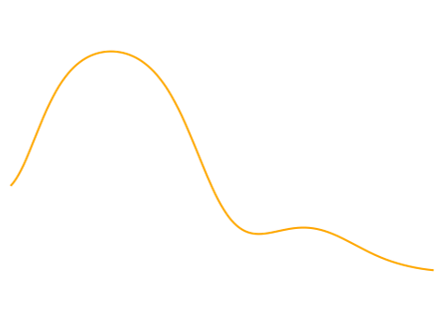
\includegraphics[width=4.8cm]{figures/funkcjacelu/R.png}};
    \draw[thick] (-0.1,3.5) node[left]{1} -- (0.1, 3.5) ;
    \draw[thick, dashed, red] (-0.1,3) node[left]{$0,98$} -- (5,3);
    \draw[->, thick] (9,0) -- (9,4) node[above]{$GDD$};
    \draw[->, thick] (9,3.5) -- (14,3.5) node[right]{$\lambda$};
    \draw[thick] (8.9,0.2) node[left, text width=2cm]{najmniejsza możliwa wartość} -- (9.1, 0.2) ;
    \draw[color=blue] (9.2,3) -- (10.2,3) -- (10.2,0.2) -- (12.8,0.2) -- (12.8,3) -- (13.8,3); 
    \node at (11.5,1.85)  {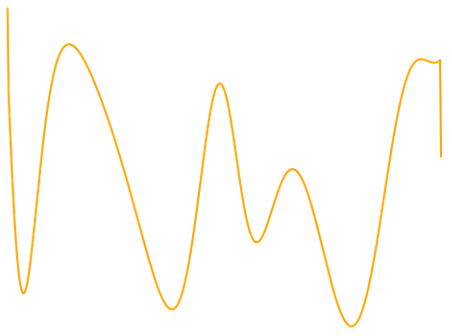
\includegraphics[width=4.8cm]{figures/funkcjacelu/gdd.png}};
    \draw[thick, dashed, red] (8.9,1.6) node[left]{średnia} -- (14,1.6);
    \draw[<->, thick, black!40!green] (11.45,2.75) -- (11.45,1.6);
    \draw[<->, thick, black!40!green] (9.85,3.18) -- (9.85,1.6);
    \draw[<->, thick, black!40!green] (10.93,0.35) -- (10.93,1.6);
   \draw[<->, thick, black!40!green] (11.83,1.06) -- (11.83,1.6);
    \end{tikzpicture}
    \caption{Warunki w funkcji celu}
    Legenda: niebieska krzywa --- funkcja oczekiwana, pomarańczowa krzywa --- funkcja rzeczywista, zielone strzałki --- odchylenie punktu od wartości średniej.
    \label{fig:idealne}
\end{figure}

Do każdego tak ustalonego parametru jest przypisywana waga, która określa w jakim stopniu dany parametr wpływa na wynik końcowy. Im dany parametr jest bliżej żądanej wartości tym bardziej funkcja celu nagradza aktualne rozwiązanie. Otrzymujemy więc 4 wagi, kolejno: $c_R$, $c_{avGDD}$, $c_{devGDD}$, $c_{ptpGDD}$.

W celu sprawdzenia poprawności tak zdefiniowanej funkcji celu, wzięto pod uwagę dwie struktury z wyraźnie różniącym się R i GDD. Dyspersyjne własności pierwszej struktury (pochodzącej z \cite{dbr1}) przedstawiono na rysunku \ref{fig:dbr1}, natomiast drugiej (pochodzącej z \cite{dbr2}) na \ref{fig:dbr2}. Można łatwo zauważyć, że w przypadku obu struktur odbijalność jest na prawidłowym poziomie, natomiast GDD w przypadku struktury 1 charakteryzuje się wyraźnym pikiem w granicach $1055\nm$. Struktura 2 natomiast charakteryzuje się GDD prawie, że stałym na poziomie $800\,\mathrm{fs^2}$. Z pełną pewnością można stwierdzić, że struktura 2 jest lepsza od struktury 1.

\begin{figure}
    \centering
    \begin{subfigure}[b]{0.46\textwidth}
        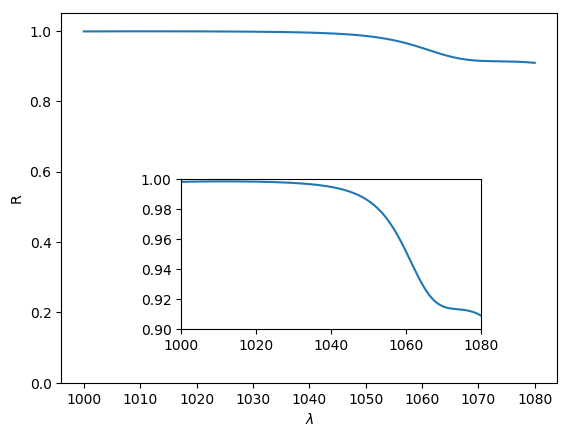
\includegraphics[width=\linewidth]{figures/funkcjacelu/result_Rdbr.png}
        \caption{R (przedstawione również w powiększeniu)}
    \end{subfigure}
       \begin{subfigure}[b]{0.49\textwidth}
        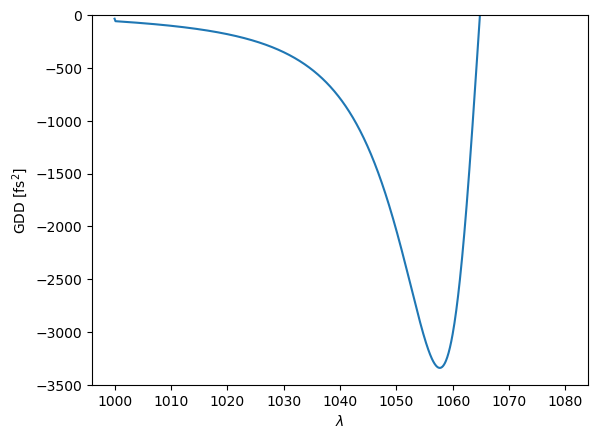
\includegraphics[width=\linewidth]{figures/funkcjacelu/result_gdddbr.png}
        \caption{GDD\\~}
    \end{subfigure}
    \caption[Dyspersyjne własności struktury 1 (gorszej)]{Dyspersyjne własności struktury 1 z \cite{dbr1} (gorszej)}
    \label{fig:dbr1}
\end{figure}

\begin{figure}
    \centering
    \begin{subfigure}[b]{0.46\textwidth}
        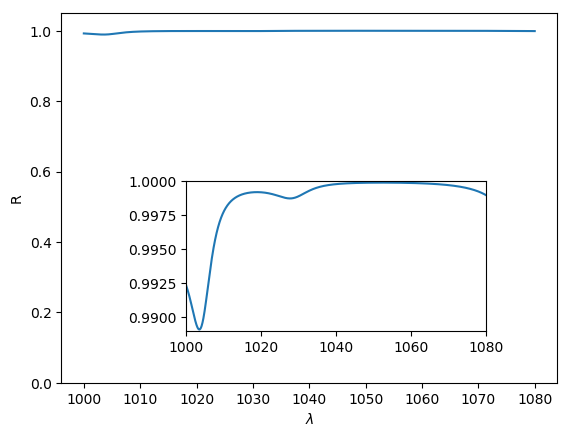
\includegraphics[width=\linewidth]{figures/funkcjacelu/result_Rdbr_opt.png}
        \caption{R (przedstawione również w powiększeniu)}
    \end{subfigure}
       \begin{subfigure}[b]{0.49\textwidth}
        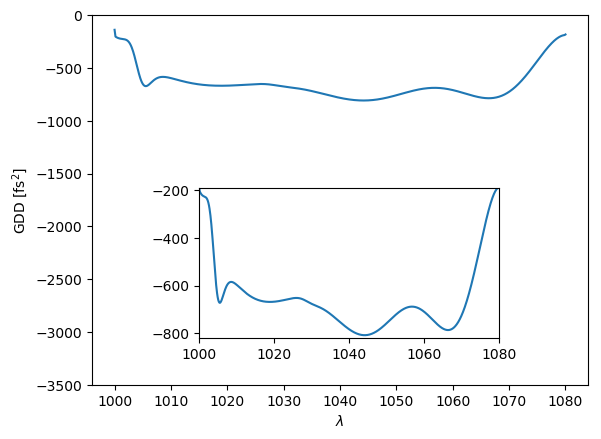
\includegraphics[width=\linewidth]{figures/funkcjacelu/result_gdddbr_opt.png}
        \caption{GDD (przedstawione również w powiększeniu)}
    \end{subfigure}
    \caption[Dyspersyjne własności struktury 2 (lepszej)]{Dyspersyjne własności struktury 2 z \cite{dbr2} (lepszej)}
    \label{fig:dbr2}
\end{figure}

Wykonano obliczenia dla dwóch różnych wartości wag i otrzymano wyniki przedstawione w tabeli \ref{tab:funkcel}.

\begin{table}[H]
    \centering
    \caption{Weryfikacja działania funkcji celu}
    \begin{tabular}{|c|c|c|c|c|c|} \cline{5-6}
        \multicolumn{4}{c}{} & \multicolumn{2}{|c|}{Wartość funkcji celu} \\\hline
         $c_R$ & $c_{avGDD}$& $c_{devGDD}$& $c_{ptpGDD}$ &  Struktura 1 (gorsza) & Struktura 2 (lepsza)\\\hline
         $0,5$ &$2$ &$10$& $1$& $69,596$ &$459,668$ \\\hline
         $100000$ & $70$& $1$& $0$& $4583.742$ & $50419.277$ \\\hline
    \end{tabular}
    \label{tab:funkcel}
\end{table}

Obserwując wyniki z tabeli \ref{tab:funkcel} widać wyraźnie, że struktura 2 dostała znacznie lepszą ocenę niż struktura 1, która została uznana za gorszą na podstawie obserwacji wykresów z rysunków \ref{fig:dbr1} i \ref{fig:dbr2}. Więc funkcja celu działa w sposób prawidłowy i można jej użyć w algorytmie rojowym. 

\section{Przedstawienie danych wejściowych i wyniki}
W celu uproszczenia problemu, założono, że zwierciadło jest zbudowane ze stałej liczby naprzemiennych warstw dwóch materiałów półprzewodnikowych: arsenku glinu AlAs oraz arsenku galu GaAs o współczynnikach załamania światła kolejno $n_1=2,956$ i $n_2=3,489$, które są również stałe podczas działania algorytmu. Dlatego też wystarczające będzie przedstawienie danych wejściowych w postaci grubości warstw do zastosowania algorytmu rojowego. Wprowadza to dużą losowość uzyskanych wyników, dlatego wykonano również obliczenia przedstawiając dane w postaci zmiennej wynikającej z warunku Bragg'a. Ponadto, sprawdzono wpływ przedstawienia danych w postaci dwóch parametrów: zmiennej wynikającej z warunku Bragg'a oraz zależności między grubościami warstw w parze. W dalszej części tekstu zostały przedstawione dokładne zależności między warstwami jakie zostały wzięte pod uwagę oraz wyniki jakie uzyskano dla każdego omawianego przypadku.

\subsection{Losowanie grubości warstw}

W pierwszej kolejności zastosowano bezpośrednio grubości warstw struktury złożonej ze 122 powłok kolejno GaAs i AlAs. Pierwsze $N$ rozwiązań jest generowane losowo w przedziale $\langle 5\nm, 1000\nm \rangle$. Otrzymane tak wyniki przedstawiono na rysunku \ref{fig:wynlosd}.

\begin{figure} [H]
    \centering
    \begin{subfigure}[b]{0.30\textwidth}
        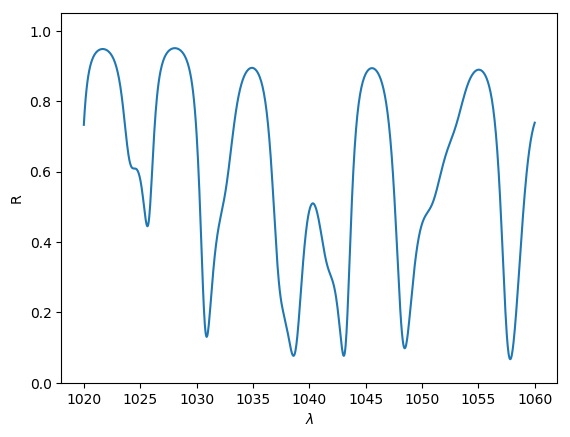
\includegraphics[width=\linewidth]{figures/wyniki/losowe/d/result_Rresult0.png}
        \caption{R w iteracji 0}
    \end{subfigure}
            \begin{subfigure}[b]{0.31\textwidth}
        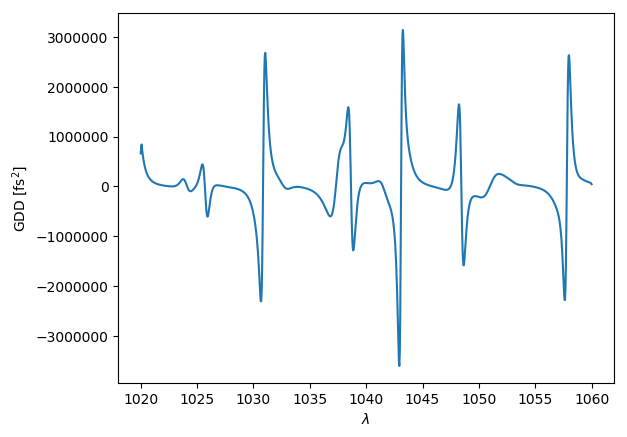
\includegraphics[width=\linewidth]{figures/wyniki/losowe/d/result_gddresult0.png}
        \caption{GDD w iteracji 0}
    \end{subfigure}
            \begin{subfigure}[b]{0.32\textwidth}
        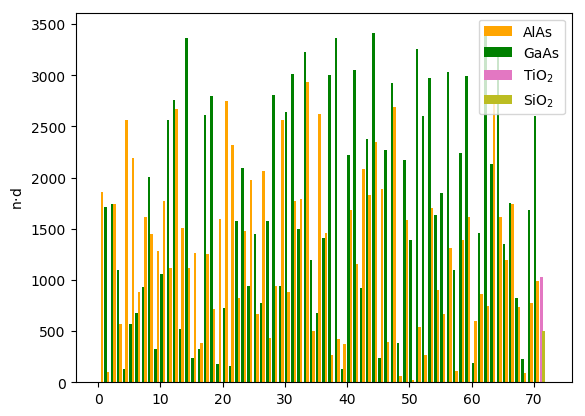
\includegraphics[width=\linewidth]{figures/wyniki/losowe/d/result_ndresult0.png}
        \caption{Iloczyn $nd$ w iteracji 0}
    \end{subfigure}
        \begin{subfigure}[b]{0.30\textwidth}
        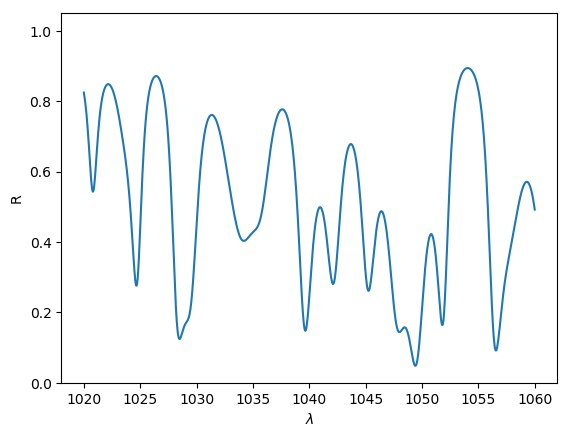
\includegraphics[width=\linewidth]{figures/wyniki/losowe/d/result_Rresult499.png}
        \caption{R w iteracji 499}
    \end{subfigure}
        \begin{subfigure}[b]{0.31\textwidth}
        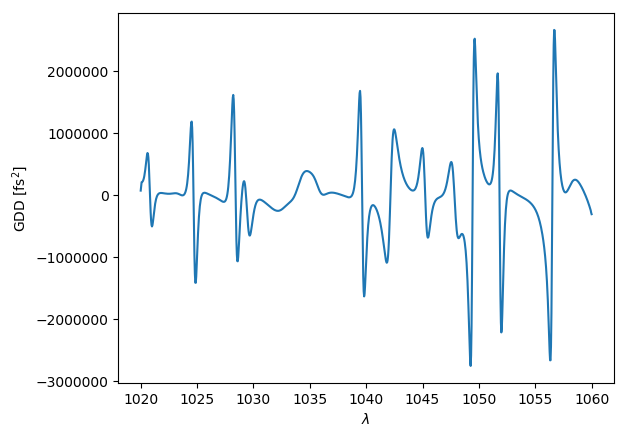
\includegraphics[width=\linewidth]{figures/wyniki/losowe/d/result_gddresult499.png}
        \caption{GDD w iteracji 499}
    \end{subfigure}
        \begin{subfigure}[b]{0.32\textwidth}
        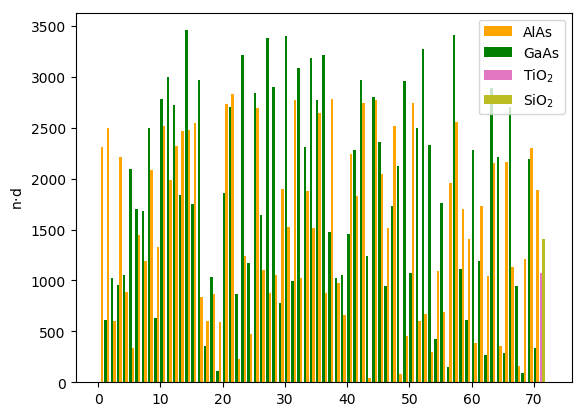
\includegraphics[width=\linewidth]{figures/wyniki/losowe/d/result_ndresult499.png}
        \caption{Iloczyn $nd$ w iteracji 499}
    \end{subfigure}
    \caption{Wyniki obliczeń w przypadku losowania grubości warstw przy rozpoczęciu obliczeń od losowo wygenerowanej struktury}
    Wartości parametrów: $N=1000$, $d_{near}= 0,005$, $w_{qual}=0,40$, $w_{best}=0,20$, $w_{better}=0,8$, $p_1=0,5$, $p_2=2$, $p_3=10$, $p_4=1$
    \label{fig:wynlosd}
\end{figure}

Można zauważyć, że wyniki wyglądają bardzo źle, ale widać jednocześnie zmianę wynikowej struktury co świadczy o działaniu programu. Można wywnioskować, że rozpoczynając obliczenia w sposób zupełnie losowy jest bardzo mało prawdopodobne znalezienie rozwiązań dobrych. Dlatego postanowiono generować pierwsze $N$ rozwiązań generując rozwiązania z dalekiego sąsiedztwa $d_{far}$ struktury już wcześniej znanej. W tym celu zostały wykorzystane struktury 1 i 2 omawiane w podrozdziale \ref{sect:cel}. Wyniki zostały przedstawione na rysunkach \ref{fig:wynlos1} i \ref{fig:wynlos2}. Parametry zostały dobrane w identyczny sposób jak w przypadku rysunku \ref{fig:wynlosd}, natomiast wartość parametru $d_{far}$ wynosi $50$.

\begin{figure} [H]
    \centering
    \begin{subfigure}[b]{0.30\textwidth}
        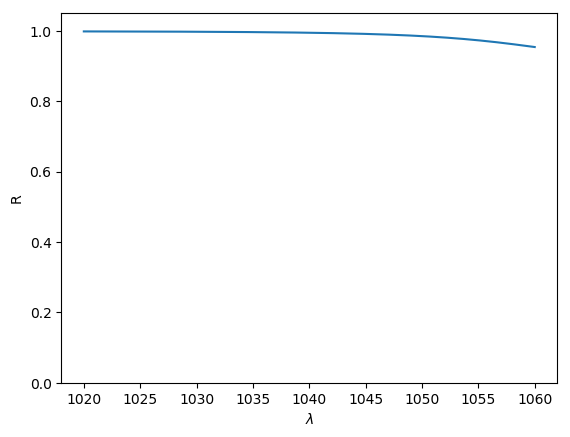
\includegraphics[width=\linewidth]{figures/wyniki/losowe/dbr/result_Rresult0.png}
        \caption{R w iteracji 0}
    \end{subfigure}
            \begin{subfigure}[b]{0.31\textwidth}
        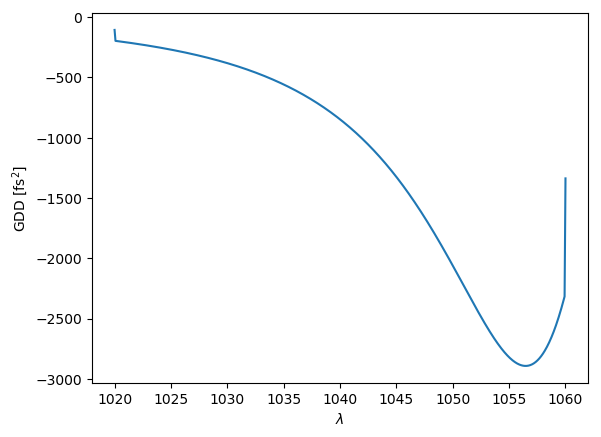
\includegraphics[width=\linewidth]{figures/wyniki/losowe/dbr/result_gddresult0.png}
        \caption{GDD w iteracji 0}
    \end{subfigure}
            \begin{subfigure}[b]{0.32\textwidth}
        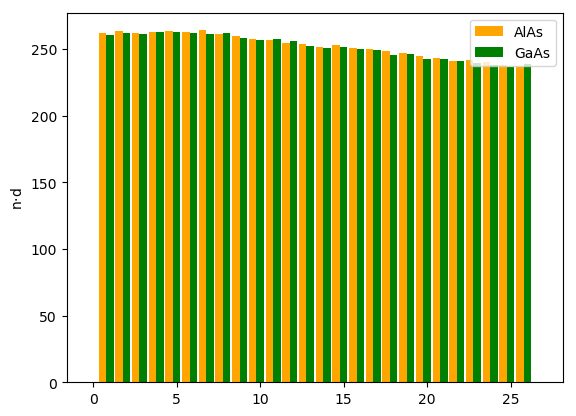
\includegraphics[width=\linewidth]{figures/wyniki/losowe/dbr/result_ndresult0.png}
        \caption{Iloczyn $nd$ w iteracji 0}
    \end{subfigure}
        \begin{subfigure}[b]{0.30\textwidth}
        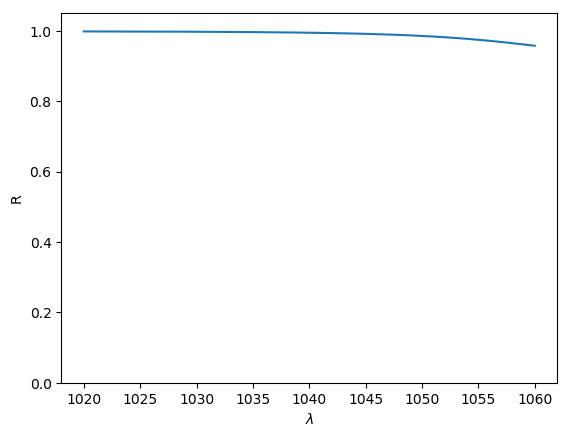
\includegraphics[width=\linewidth]{figures/wyniki/losowe/dbr/result_Rresult499.png}
        \caption{R w iteracji 499}
    \end{subfigure}
        \begin{subfigure}[b]{0.31\textwidth}
        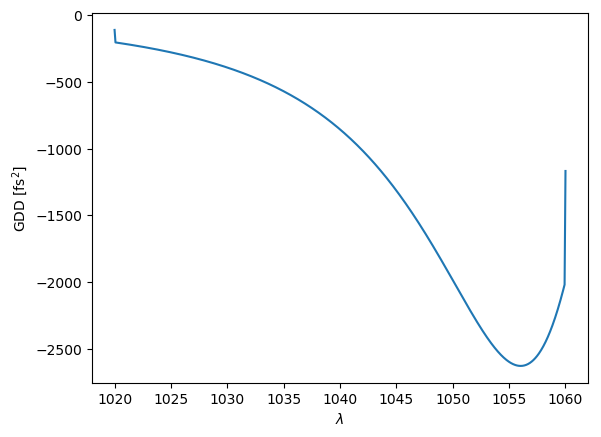
\includegraphics[width=\linewidth]{figures/wyniki/losowe/dbr/result_gddresult499.png}
        \caption{GDD w iteracji 499}
    \end{subfigure}
        \begin{subfigure}[b]{0.32\textwidth}
        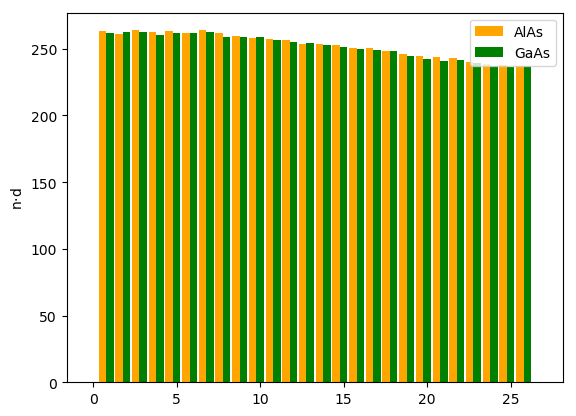
\includegraphics[width=\linewidth]{figures/wyniki/losowe/dbr/result_ndresult499.png}
        \caption{Iloczyn $nd$ w iteracji 499}
    \end{subfigure}
    \caption{Wyniki obliczeń w przypadku losowania grubości warstw przy rozpoczęciu obliczeń od struktury 1 (gorszej)}
    \label{fig:wynlos1}
\end{figure}

\begin{figure} [H]
    \centering
    \begin{subfigure}[b]{0.30\textwidth}
        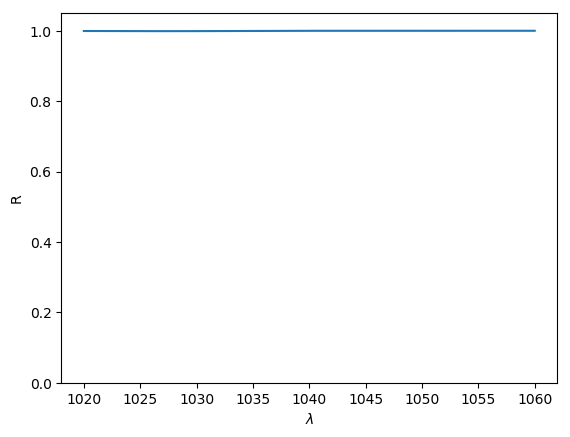
\includegraphics[width=\linewidth]{figures/wyniki/losowe/dbr_opt/result_Rresult0.png}
        \caption{R w iteracji 0}
    \end{subfigure}
            \begin{subfigure}[b]{0.31\textwidth}
        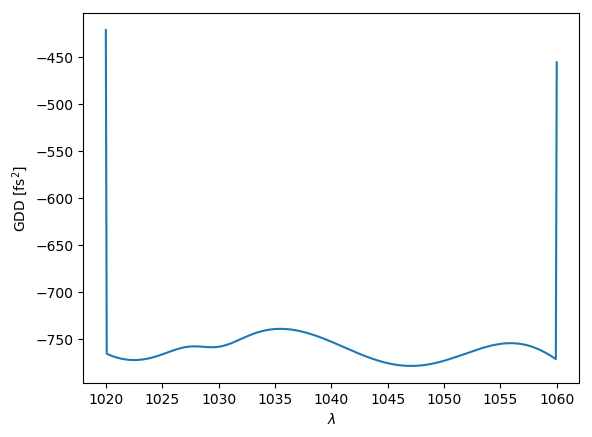
\includegraphics[width=\linewidth]{figures/wyniki/losowe/dbr_opt/result_gddresult0.png}
        \caption{GDD w iteracji 0}
    \end{subfigure}
            \begin{subfigure}[b]{0.32\textwidth}
        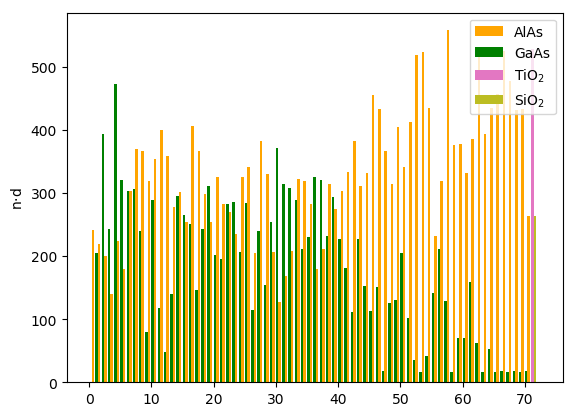
\includegraphics[width=\linewidth]{figures/wyniki/losowe/dbr_opt/result_ndresult0.png}
        \caption{Iloczyn $nd$ w iteracji 0}
    \end{subfigure}
        \begin{subfigure}[b]{0.30\textwidth}
        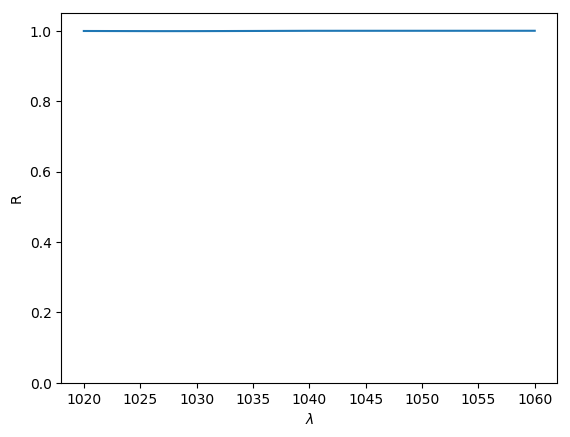
\includegraphics[width=\linewidth]{figures/wyniki/losowe/dbr_opt/result_Rresult499.png}
        \caption{R w iteracji 499}
    \end{subfigure}
        \begin{subfigure}[b]{0.31\textwidth}
        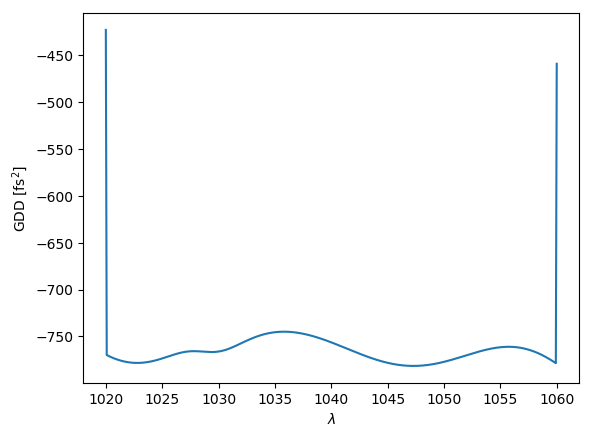
\includegraphics[width=\linewidth]{figures/wyniki/losowe/dbr_opt/result_gddresult499.png}
        \caption{GDD w iteracji 499}
    \end{subfigure}
        \begin{subfigure}[b]{0.32\textwidth}
        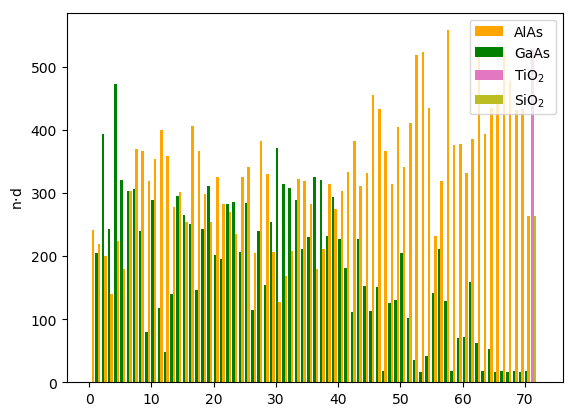
\includegraphics[width=\linewidth]{figures/wyniki/losowe/dbr_opt/result_ndresult499.png}
        \caption{Iloczyn $nd$ w iteracji 499}
    \end{subfigure}
    \caption{Wyniki obliczeń w przypadku losowania grubości warstw przy rozpoczęciu obliczeń od struktury 2 (lepszej)}
    \label{fig:wynlos2}
\end{figure}
\newpage
Można zauważyć, że dla lepszej struktury otrzymano wyniki zdecydowanie lepsze, co dowodzi, że to jest dobry sposób na lekkie polepszenie już istniejącej struktury, jednocześnie nie umożliwiając stworzenia nowej struktury zupełnie od zera. Dodatkowo można zauważyć, że w przypadku \ref{fig:wynlos2} najlepsza struktura nie zmieniła się po 499 iteracjach, co ilustruje trudność otrzymania w ten sposób rozwiązań naprawdę dobrych.

Dodatkowo powtórzono obliczenia z rysunku \ref{fig:wynlos2}, lecz wykorzystując tym razem 100 razy większą ilości pszczół zwiadowców przy mniejszej ilości iteracji (ze względu na ich znaczącą długość). Otrzymane wyniki przedstawiono na rysunku \ref{fig:wynlos3}. Można zauważyć, że różnice między otrzymanymi wykresami nie są znaczące i zmiana tego parametru nie ma wpływu na wynik w tym wypadku.

\begin{figure} [H]
    \centering
    \begin{subfigure}[b]{0.30\textwidth}
        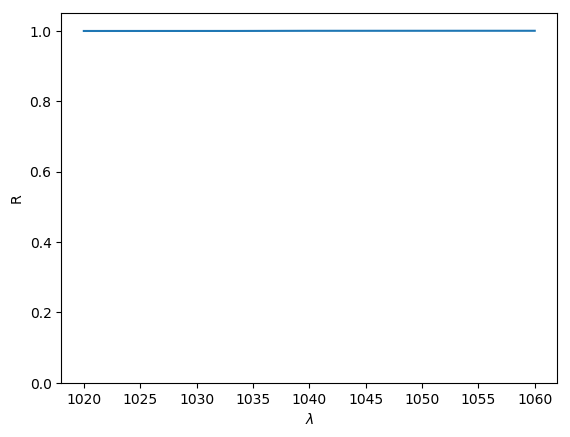
\includegraphics[width=\linewidth]{figures/wyniki/losowe/dbr_opt10/result_Rresult0.png}
        \caption{R w iteracji 0}
    \end{subfigure}
            \begin{subfigure}[b]{0.31\textwidth}
        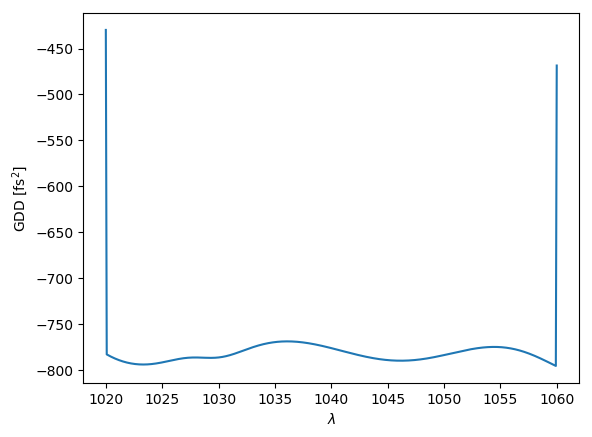
\includegraphics[width=\linewidth]{figures/wyniki/losowe/dbr_opt10/result_gddresult0.png}
        \caption{GDD w iteracji 0}
    \end{subfigure}
            \begin{subfigure}[b]{0.32\textwidth}
        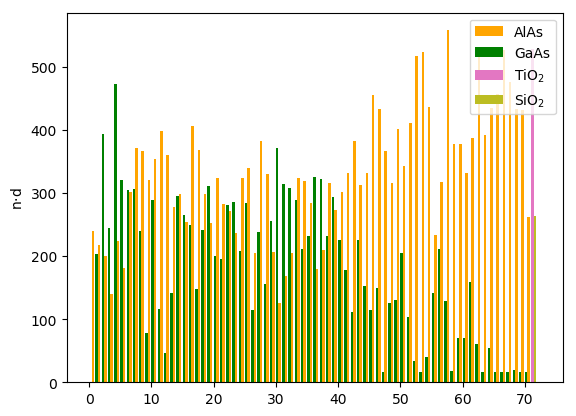
\includegraphics[width=\linewidth]{figures/wyniki/losowe/dbr_opt10/result_ndresult0.png}
        \caption{Iloczyn $nd$ w iteracji 0}
    \end{subfigure}
        \begin{subfigure}[b]{0.30\textwidth}
        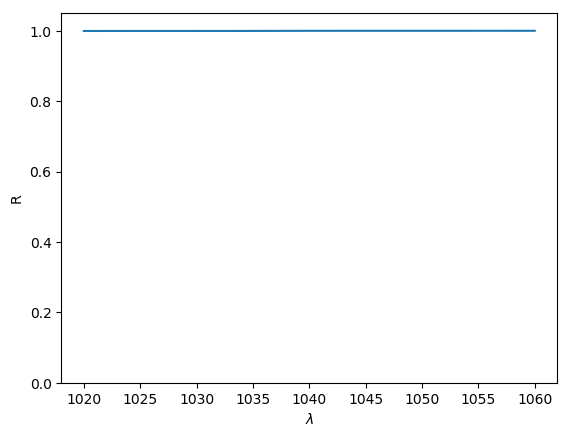
\includegraphics[width=\linewidth]{figures/wyniki/losowe/dbr_opt10/result_Rresult10.png}
        \caption{R w iteracji 10}
    \end{subfigure}
        \begin{subfigure}[b]{0.31\textwidth}
        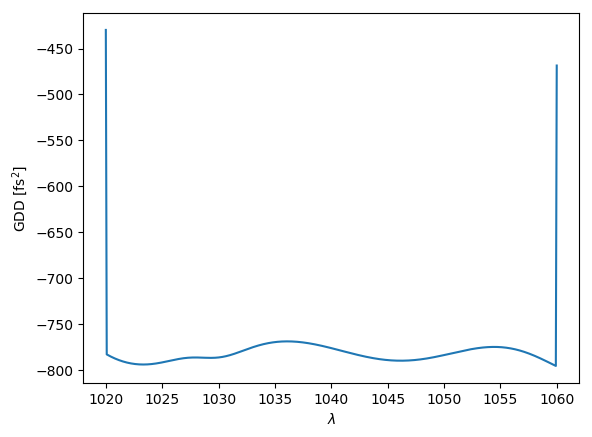
\includegraphics[width=\linewidth]{figures/wyniki/losowe/dbr_opt10/result_gddresult10.png}
        \caption{GDD w iteracji 10}
    \end{subfigure}
        \begin{subfigure}[b]{0.32\textwidth}
        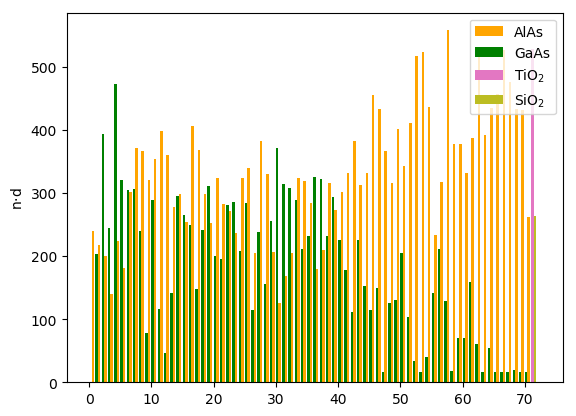
\includegraphics[width=\linewidth]{figures/wyniki/losowe/dbr_opt10/result_ndresult10.png}
        \caption{Iloczyn $nd$ w iteracji 10}
    \end{subfigure}
    \caption{Wyniki obliczeń w przypadku losowania grubości warstw przy rozpoczęciu obliczeń od struktury 2 (lepszej) i $N = 100000$ pszczół}
    \label{fig:wynlos3}
\end{figure}

\subsection{Losowanie parametru wykorzystującego warunek Bragg'a} % df = n_warstw - n_warstw/2
Następnie, aby polepszyć uzyskiwanie wyniki i zminimalizować losowość, skorzystano z warunku Bragg'a:
\begin{equation}
    n_1d_1 + n_2d_2 = \frac{\lambda_B}{2}, \label{eq:bragg}
\end{equation}
gdzie $n_1$, $n_2$ --- współczynniki załamania warstw $1$ i $2$, $d_1$, $d_2$ --- grubości warstw $1$ i $2$, $\lambda_B$ --- długość fali Bragg'a czyli długość fali dla której zwierciadło osiąga maksimum odbijalności. Warunek ten posłużył do wprowadzenia zmiennej $c$, zdefiniowanej według wzoru:
\begin{equation}
    \lambda_B = \lambda c. \label{eq:c}
\end{equation}
Wartość $\lambda$ oznacza środek właśnie badanego przedziału długości fali. Tak dobrana zmienna $c$ oscyluje w przedziale $\langle 0,5, 1,5 \rangle$, a co za tym idzie $\lambda_B$ przyjmuje wartości od $500\nm$ do $1500\nm$ przy $\lambda = 1000\nm$. Dodatkowo wprowadzono warunek na zachowanie równości iloczynu $nd$ dla każdej z warstw w danej parze, zgodnie ze wzorem $n_1d_1=n_2d_2$. Na tej podstawie otrzymano następujące wzory na grubości warstw w parze: 

\begin{equation}
    \left\{ \begin{array}{c}
         d_1 = \frac{c\lambda}{4n_1}, \\ d_2 = \frac{c\lambda}{4n_2},
    \end{array}\right.
\end{equation}
natomiast wartość $c$ można obliczyć podstawiając \ref{eq:c} do \ref{eq:bragg}, co daje następujące równanie:
\begin{equation}
    c = \frac{2}{\lambda} \cdot (n_1d_1 + n_2d_2).
\end{equation}
Tak otrzymane równania posłużyły do stworzenia funkcji konwersji z grubości warstw do zmiennej $c$ i w odwrotnym kierunku. W tym momencie możliwe było już zastosowanie zmiennej $c$ w algorytmie rojowym. Tak też zostało zrobione i po licznym próbach korzystając z różnych wartości wag funkcji celu, udało się uzyskać wyniki przedstawione na rysunku \ref{fig:wyn1stp} korzystając ze współczynników załamania struktury 1 (gorszej). Dodatkowo wykonano dla tych samych parametrów następne obliczenia na rysunku \ref{fig:wyn1stpopt1} tym razem korzystając z zestawu współczynników odbicia ze struktury 2 (lepszej). Na koniec wykonano jeszcze obliczenia zwiększając liczbę pszczół zwiadowców 100 krotnie względem \ref{fig:wyn1stpopt1} i przedstawiono wyniki na rysunku \ref{fig:wyn1stpopt2}.


\begin{figure} [ht!]
    \centering
    \begin{subfigure}[b]{0.30\textwidth}
        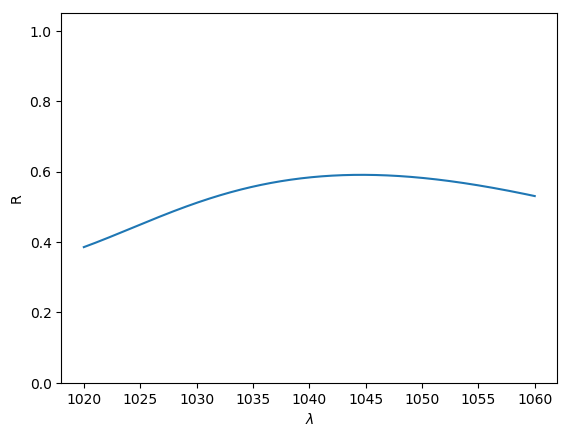
\includegraphics[width=\linewidth]{figures/wyniki/1stopien/fcelptp/result_R0.png}
        \caption{R w iteracji 0}
    \end{subfigure}
            \begin{subfigure}[b]{0.31\textwidth}
        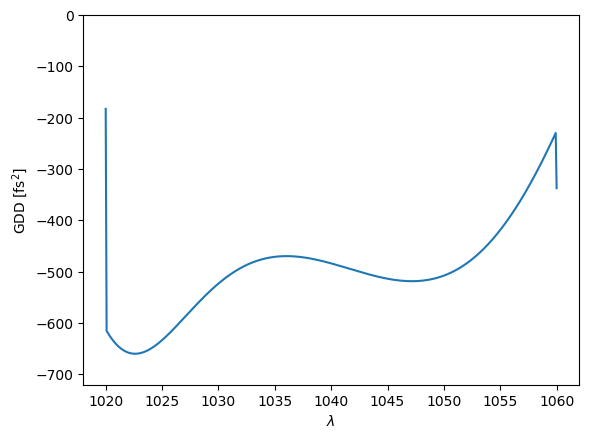
\includegraphics[width=\linewidth]{figures/wyniki/1stopien/fcelptp/result_gdd0.png}
        \caption{GDD w iteracji 0}
    \end{subfigure}
        \begin{subfigure}[b]{0.32\textwidth}
        \includegraphics[width=\linewidth]{figures/wyniki/1stopien/fcelptp/result_nd0.png}
        \caption{Iloczyn $nd$ w iteracji 0}
    \end{subfigure}
        \begin{subfigure}[b]{0.30\textwidth}
        \includegraphics[width=\linewidth]{figures/wyniki/1stopien/fcelptp/result_R1.png}
        \caption{R w iteracji 499}
    \end{subfigure}
        \begin{subfigure}[b]{0.31\textwidth}
        \includegraphics[width=\linewidth]{figures/wyniki/1stopien/fcelptp/result_gdd1.png}
        \caption{GDD w iteracji 499}
    \end{subfigure}
        \begin{subfigure}[b]{0.32\textwidth}
        \includegraphics[width=\linewidth]{figures/wyniki/1stopien/fcelptp/result_nd1.png}
        \caption{Iloczyn $nd$ w iteracji 499}
    \end{subfigure}
    \caption{Wyniki obliczeń w przypadku losowania parametru wykorzystującego warunek Bragg'a przy wykorzystaniu współczynników załamania ze struktury 1}
    Wartości parametrów: $N= 1000$, $d_{near}= 0,005$, $w_{qual}=0,40$, $w_{best}=0,20$, $w_{better}=0,8$, $p_1=0,5$, $p_2=2$, $p_3=10$, $p_4=1$
    \label{fig:wyn1stp}
\end{figure}

Można zauważyć na podstawie przedstawionych wyników, że otrzymane wyniki są gorsze od uzyskanego na rysunku \ref{fig:wynlos2}. Dodatkowo iloczyny $nd$ dla każdej warstwy z danej pary są równe, co świadczy o działaniu programu w sposób pożądany. Dodatkowo można zaobserwować ciekawy rezultat --- wyniki korzystające ze struktury teoretycznie gorszej dały zauważalnie lepszy wynik niż te korzystające ze struktury teoretycznie lepszej. Oprócz tego widać, że obliczenia przy większej ilości pszczół zwiadowców (rysunek \ref{fig:wyn1stpopt2} dają gorsze rezultaty niż te przy mniejszej ich ilości (rysunek \ref{fig:wyn1stpopt1}), w odróżnieniu od podejścia korzystającego z samych grubości warstw.

\begin{figure} [H]
    \centering
    \begin{subfigure}[b]{0.30\textwidth}
        \includegraphics[width=\linewidth]{figures/wyniki/1stopien/opt1000/result_Rresult0.png}
        \caption{R w iteracji 0}
    \end{subfigure}
            \begin{subfigure}[b]{0.31\textwidth}
        \includegraphics[width=\linewidth]{figures/wyniki/1stopien/opt1000/result_gddresult0.png}
        \caption{GDD w iteracji 0}
    \end{subfigure}
            \begin{subfigure}[b]{0.32\textwidth}
        \includegraphics[width=\linewidth]{figures/wyniki/1stopien/opt1000/result_ndresult0.png}
        \caption{Iloczyn $nd$ w iteracji 0}
    \end{subfigure}
        \begin{subfigure}[b]{0.30\textwidth}
        \includegraphics[width=\linewidth]{figures/wyniki/1stopien/opt1000/result_Rresult499.png}
        \caption{R w iteracji 499}
    \end{subfigure}
        \begin{subfigure}[b]{0.31\textwidth}
        \includegraphics[width=\linewidth]{figures/wyniki/1stopien/opt1000/result_gddresult499.png}
        \caption{GDD w iteracji 499}
    \end{subfigure}
        \begin{subfigure}[b]{0.32\textwidth}
        \includegraphics[width=\linewidth]{figures/wyniki/1stopien/opt1000/result_ndresult499.png}
        \caption{Iloczyn $nd$ w iteracji 499}
    \end{subfigure}
    \caption{Wyniki obliczeń w przypadku losowania parametru wykorzystującego warunek Bragg'a przy wykorzystaniu współczynników załamania ze struktury 2}
    Wartości parametrów: $N= 1000$, $d_{near}= 0,005$, $w_{qual}=0,40$, $w_{best}=0,20$, $w_{better}=0,8$, $p_1=0,5$, $p_2=2$, $p_3=10$, $p_4=1$
    \label{fig:wyn1stpopt1}
\end{figure}

\begin{figure} [H]
    \centering
    \begin{subfigure}[b]{0.30\textwidth}
        \includegraphics[width=\linewidth]{figures/wyniki/1stopien/opt10^5/result_Rresult0.png}
        \caption{R w iteracji 0}
    \end{subfigure}
            \begin{subfigure}[b]{0.31\textwidth}
        \includegraphics[width=\linewidth]{figures/wyniki/1stopien/opt10^5/result_gddresult0.png}
        \caption{GDD w iteracji 0}
    \end{subfigure}
            \begin{subfigure}[b]{0.32\textwidth}
        \includegraphics[width=\linewidth]{figures/wyniki/1stopien/opt10^5/result_ndresult0.png}
        \caption{Iloczyn $nd$ w iteracji 0}
    \end{subfigure}
        \begin{subfigure}[b]{0.30\textwidth}
        \includegraphics[width=\linewidth]{figures/wyniki/1stopien/opt10^5/result_Rresult10.png}
        \caption{R w iteracji 10}
    \end{subfigure}
        \begin{subfigure}[b]{0.31\textwidth}
        \includegraphics[width=\linewidth]{figures/wyniki/1stopien/opt10^5/result_gddresult10.png}
        \caption{GDD w iteracji 10}
    \end{subfigure}
        \begin{subfigure}[b]{0.32\textwidth}
        \includegraphics[width=\linewidth]{figures/wyniki/1stopien/opt10^5/result_ndresult10.png}
        \caption{Iloczyn $nd$ w iteracji 10}
    \end{subfigure}
    \caption{Wyniki obliczeń w przypadku losowania parametru wykorzystującego warunek Bragg'a przy wykorzystaniu współczynników załamania ze struktury 2}
    Wartości parametrów: $N= 100000$, $d_{near}= 0,005$, $w_{qual}=0,40$, $w_{best}=0,20$, $w_{better}=0,8$, $p_1=0,5$, $p_2=2$, $p_3=10$, $p_4=1$
    \label{fig:wyn1stpopt2}
\end{figure}

\subsection{Losowanie 2 parametrów korzystając z warunku Bragg'a i zależności między grubościami warstw} % df = n_warstw - n_warstw
Na koniec, inspirując się pracą \cite{dbr2}, gdzie z sukcesem udało się znaleźć dobre wyniki zarówno dla GDD i R korzystając z algorytmów genetycznych i prezentując dane w postaci dwóch parametrów: jeden zależny od warunku Bragg'a jak w przypadku poprzednim a drugi wprowadzający zależność między iloczynami $nd$ dla warstw w każdej parze, postanowiono sprawdzić czy również w przypadku algorytmów rojowych ta reprezentacja da rónie dobre wyniki. W tym celu zastosowano następujący układ równań:
\begin{equation}
    \left\{\begin{array}{l}
         n_1d_1 + n_2d_2 = \frac{\lambda_B}{2},  \\
         n_1d_1=h(n_1d_1 + n_2d_2) = h \cdot\frac{\lambda_B}{2}, \\
          n_2d_2=(1-h)(n_1d_1 + n_2d_2) = (1-h) \cdot\frac{\lambda_B}{2}, \\
          \lambda_B=\lambda\left[1+s\left(c-\frac 12\right)\right],
    \end{array}\right.
\end{equation}
gdzie: c, h --- zmienne przyjmujące wartości z zakresu $\langle0, 1\rangle$, które będą używane w algorytmie rojowym jako argument badanej funkcji (jedna para tych wartości odpowiada parze w strukturze DBR), s --- parametr pozwalający określić zakres wartości jakie przyjmuje $\lambda_B$. \\
Korzystając z tak przygotowanego układu równań, można wyznaczyć grubości warstw w danej parze:
\begin{equation}
    \left\{ \begin{array}{l}
         d_1 = \displaystyle\frac{h\lambda_B}{2n_1}, \\ d_2 = \displaystyle\frac{(1-h)\lambda_B}{2n_2}.
    \end{array}\right.
\end{equation}
Na podstawie tych wzorów sporządzono funkcję umożliwiającą transformację tablicy zmiennych $c$ i $h$ w tablicę grubości warstw w zwierciadle. Dodatkowo można było sporządzić funkcję odwrotną poprzez wyznaczenie wartości $c$ i $h$ zgodnie z:
\begin{equation}
    \left\{\begin{array}{l}
          c = \displaystyle\frac{2}{\lambda s}(n_1d_1 + n_2d_2) - \frac 1s + \frac 12, \\
           h = 1 + \displaystyle\frac{n_2d_2}{n_1d_1}.
    \end{array}\right.
\end{equation}

Na podstawie tak wyznaczonych zmiennych i funkcji dokonano obliczeń dla wielu zestawów parametrów funkcji celu. Najlepsze wyniki jakie udało się uzyskać przy użyciu współczynników załamania ze struktury 1 omawianej w \ref{sect:cel} przedstawiono na rysunku \ref{fig:wyn2stp1}, natomiast te przy użyciu współczynników załamania ze struktury 2 przedstawiono na rysunku \ref{fig:wyn2stp2}. Dodatkowo postanowiono sprawdzić, również tutaj, wpływ zmiany ilości zwiadowców na wynik. W tym celu przyjęto $N=100000$ i wykonano obliczenia, których rezultat został przedstawiony na rysunku \ref{fig:wyn2stp3}.

Można zauważyć, że wyniki przedstawione na rysunkach \ref{fig:wyn2stp1}, \ref{fig:wyn2stp2} i \ref{fig:wyn2stp3} są znacznie gorsze od wyników otrzymanych w poprzednich podejściach. Natomiast porównując je bezpośrednio do siebie, można zauważyć, że zmiana ilości par zwierciadeł DBR i wprowadzenie dodatkowych warstw z innych materiałów półprzewodnikowych znaczącą polepszyło rozwiązania na rysunku \ref{fig:wyn2stp2} względem \ref{fig:wyn2stp1}. Ponadto widać, że w tym wypadku, zwiększenie liczby pszczół zwiadowców nie wpłynęło szczególnie na jakość otrzymanego rozwiązania, natomiast zauważalnie przyspieszyło proces wyznaczenia rozwiązania finalnego, gdyż na rysunku \ref{fig:wyn2stp3} widać, że wykresy dla iteracji 0 jak i 10 są identyczne. Podsumowując, wyniki w przypadku algorytmu rojowego nie zyskują na jakości po wprowadzeniu tego sposobu reprezentacji danych, w odróżnieniu do algorytmów genetycznych. Możliwym sposobem na polepszenie wyników jest dopuszczenie zmiany ilości par zwierciadeł jak i dopuszczenie dodania dodatkowych warstw na koniec z innych materiałów. Takie rozwiązanie niestety nie zostało sprawdzone.

\begin{figure} [ht!]
    \centering
    \begin{subfigure}[b]{0.30\textwidth}
        \includegraphics[width=\linewidth]{figures/wyniki/2stopien/dbr/result_Rresult0.png}
        \caption{R w iteracji 0}
    \end{subfigure}
            \begin{subfigure}[b]{0.31\textwidth}
        \includegraphics[width=\linewidth]{figures/wyniki/2stopien/dbr/result_gddresult0.png}
        \caption{GDD w iteracji 0}
    \end{subfigure}
        \begin{subfigure}[b]{0.32\textwidth}
        \includegraphics[width=\linewidth]{figures/wyniki/2stopien/dbr/result_ndresult0.png}
        \caption{Iloczyn $nd$ w iteracji 0}
    \end{subfigure}
        \begin{subfigure}[b]{0.30\textwidth}
        \includegraphics[width=\linewidth]{figures/wyniki/2stopien/dbr/result_Rresult499.png}
        \caption{R w iteracji 499}
    \end{subfigure}
        \begin{subfigure}[b]{0.31\textwidth}
        \includegraphics[width=\linewidth]{figures/wyniki/2stopien/dbr/result_gddresult499.png}
        \caption{GDD w iteracji 499}
    \end{subfigure}
        \begin{subfigure}[b]{0.32\textwidth}
        \includegraphics[width=\linewidth]{figures/wyniki/2stopien/dbr/result_ndresult499.png}
        \caption{Iloczyn $nd$ w iteracji 499}
    \end{subfigure}
    \caption{Wyniki obliczeń w przypadku losowania 2 parametrów przy wykorzystaniu współczynników załamania ze struktury 1}
    Wartości parametrów: $N= 1000$, $d_{near}= 0,05$, $w_{qual}=0,2$, $w_{best}=0,2$, $w_{better}=0,8$, $p_1=0.5$, $p_2=2$, $p_3=10$, $p_4=1$, $s=0.038$
    \label{fig:wyn2stp1}
\end{figure}

\begin{figure} [H]
    \centering
    \begin{subfigure}[b]{0.30\textwidth}
        \includegraphics[width=\linewidth]{figures/wyniki/2stopien/result_Rresult0.png}
        \caption{R w iteracji 0}
    \end{subfigure}
            \begin{subfigure}[b]{0.31\textwidth}
        \includegraphics[width=\linewidth]{figures/wyniki/2stopien/result_gddresult0.png}
        \caption{GDD w iteracji 0}
    \end{subfigure}
        \begin{subfigure}[b]{0.32\textwidth}
        \includegraphics[width=\linewidth]{figures/wyniki/2stopien/result_ndresult0.png}
        \caption{Iloczyn $nd$ w iteracji 0}
    \end{subfigure}
        \begin{subfigure}[b]{0.30\textwidth}
        \includegraphics[width=\linewidth]{figures/wyniki/2stopien/result_Rresult499.png}
        \caption{R w iteracji 499}
    \end{subfigure}
        \begin{subfigure}[b]{0.31\textwidth}
        \includegraphics[width=\linewidth]{figures/wyniki/2stopien/result_gddresult499.png}
        \caption{GDD w iteracji 499}
    \end{subfigure}
        \begin{subfigure}[b]{0.32\textwidth}
        \includegraphics[width=\linewidth]{figures/wyniki/2stopien/result_ndresult499.png}
        \caption{Iloczyn $nd$ w iteracji 499}
    \end{subfigure}
    \caption{Wyniki obliczeń w przypadku losowania 2 parametrów przy wykorzystaniu współczynników załamania ze struktury 2}
    Wartości parametrów: $N= 1000$, $d_{near}= 0,005$, $w_{qual}=0,4$, $w_{best}=0,2$, $w_{better}=0,8$, $p_1=10$, $p_2=20$, $p_3=10$, $p_4=5$, $s=0.038$
    \label{fig:wyn2stp2}
\end{figure}

\begin{figure} [H]
    \centering
    \begin{subfigure}[b]{0.30\textwidth}
        \includegraphics[width=\linewidth]{figures/wyniki/2stopien/morebees/result_Rresult0.png}
        \caption{R w iteracji 0}
    \end{subfigure}
            \begin{subfigure}[b]{0.31\textwidth}
        \includegraphics[width=\linewidth]{figures/wyniki/2stopien/morebees/result_gddresult0.png}
        \caption{GDD w iteracji 0}
    \end{subfigure}
        \begin{subfigure}[b]{0.32\textwidth}
        \includegraphics[width=\linewidth]{figures/wyniki/2stopien/morebees/result_ndresult0.png}
        \caption{Iloczyn $nd$ w iteracji 0}
    \end{subfigure}
        \begin{subfigure}[b]{0.30\textwidth}
        \includegraphics[width=\linewidth]{figures/wyniki/2stopien/morebees/result_Rresult10.png}
        \caption{R w iteracji 10}
    \end{subfigure}
        \begin{subfigure}[b]{0.31\textwidth}
        \includegraphics[width=\linewidth]{figures/wyniki/2stopien/morebees/result_gddresult10.png}
        \caption{GDD w iteracji 10}
    \end{subfigure}
        \begin{subfigure}[b]{0.32\textwidth}
        \includegraphics[width=\linewidth]{figures/wyniki/2stopien/morebees/result_ndresult10.png}
        \caption{Iloczyn $nd$ w iteracji 10}
    \end{subfigure}
    \caption{Wyniki obliczeń w przypadku losowania 2 parametrów przy wykorzystaniu współczynników załamania ze struktury 2}
    Wartości parametrów: $N= 100000$, $d_{near}= 0,005$, $w_{qual}=0,4$, $w_{best}=0,2$, $w_{better}=0,8$, $p_1=10$, $p_2=20$, $p_3=10$, $p_4=5$, $s=0.038$
    \label{fig:wyn2stp3}
\end{figure}

\section{Zastosowane technologie informatyczne}

Pod koniec tego rozdziału należy jeszcze odpowiedzieć na pytanie jakie technologie zostały wykorzystane przy pisaniu programu jak i przy samym liczeniu. 
Program został napisany w języku \textit{Python 3} z wykorzystaniem biblioteki \textit{numpy} do wykonywania obliczeń na macierzach oraz \textit{matplotplib} do wykonywania wykresów.

Cały algorytm podczas jednego cyklu wykonywał ok. miliona obliczeń trwających ok. $0,40\,$s każde, co skutkowało trudnością w uruchomienia go na komputerze osobistym ze względu na małą moc obliczeniową i co za tym idzie bardzo bardzo długim czasie wykonywania obliczeń (ponad 111 godzin). Dlatego też skorzystano z klastrów komputerowych pod nazwą \textit{Dragon} i \textit{Hydra} należących do Zespołu Fotoniki Instytutu Fizyki Politechniki Łódzkiej, co umożliwiło znaczne skrócenie obliczeń, do około 3 godzin przy wykorzystaniu 48 wątków na klastrze.

W celu wykorzystania dobrodziejstw klastra zastosowano bibliotekę \textit{mpi4py}, która pozwoliła na podział danych na poszczególne wątki i wykonywania obliczeń niezależnie. Później pod koniec każdej iteracji dane są zbierane do jednego wątku w celu podsumowania otrzymanych wyników.

Podsumowując udało się, z sukcesem, zastosować algorytmy rojowe w celu znalezienia zwierciadła DBR oferującego jak najmniejszą możliwą dyspersję opróżnienia grupowego. Niestety otrzymane wyniki są zauważalne gorsze od tych znajdujących się w literaturze (np. w \cite{dbr2}), lecz metoda ta pokazuje zauważalny potencjał. 
%W celu uproszczenia problemu, założono, że zwierciadło jest zbudowane ze stałej liczby naprzemiennych warstw dwóch materiałów półprzewodnikowych: arsenku glinu AlAs oraz arsenku galu GaAs o współczynnikach załamania światła kolejno $n_1=2,956$ i $n_2=3,489$, które są również stałe podczas działania algorytmu. Dlatego też wystarczające będzie przedstawienie danych wejściowych w postaci grubości warstw do zastosowania algorytmu rojowego. Wprowadza to dużą losowość uzyskanych wyników, dlatego wykonano również obliczenia przedstawiając dane w postaci zmiennej wynikającej z warunku Bragg'a. Ponadto, sprawdzono wpływ przedstawienia danych w postaci dwóch parametrów: zmiennej wynikającej z warunku Bragg'a oraz zależności między grubościami warstw w parze. W dalszej części tekstu zostały przedstawione dokładne zależności między warstwami jakie zostały wzięte pod uwagę oraz wyniki jakie uzyskano dla każdego omawianego przypadku.

\subsection{Losowanie grubości warstw}

W pierwszej kolejności zastosowano bezpośrednio grubości warstw struktury złożonej ze 122 powłok kolejno GaAs i AlAs. Pierwsze $N$ rozwiązań jest generowane losowo w przedziale $\langle 5\nm, 1000\nm \rangle$. Otrzymane tak wyniki przedstawiono na rysunku \ref{fig:wynlosd}.

\begin{figure} [H]
    \centering
    \begin{subfigure}[b]{0.30\textwidth}
        \includegraphics[width=\linewidth]{figures/wyniki/losowe/d/result_Rresult0.png}
        \caption{R w iteracji 0}
    \end{subfigure}
            \begin{subfigure}[b]{0.31\textwidth}
        \includegraphics[width=\linewidth]{figures/wyniki/losowe/d/result_gddresult0.png}
        \caption{GDD w iteracji 0}
    \end{subfigure}
            \begin{subfigure}[b]{0.32\textwidth}
        \includegraphics[width=\linewidth]{figures/wyniki/losowe/d/result_ndresult0.png}
        \caption{Iloczyn $nd$ w iteracji 0}
    \end{subfigure}
        \begin{subfigure}[b]{0.30\textwidth}
        \includegraphics[width=\linewidth]{figures/wyniki/losowe/d/result_Rresult499.png}
        \caption{R w iteracji 499}
    \end{subfigure}
        \begin{subfigure}[b]{0.31\textwidth}
        \includegraphics[width=\linewidth]{figures/wyniki/losowe/d/result_gddresult499.png}
        \caption{GDD w iteracji 499}
    \end{subfigure}
        \begin{subfigure}[b]{0.32\textwidth}
        \includegraphics[width=\linewidth]{figures/wyniki/losowe/d/result_ndresult499.png}
        \caption{Iloczyn $nd$ w iteracji 499}
    \end{subfigure}
    \caption{Wyniki obliczeń w przypadku losowania grubości warstw przy rozpoczęciu obliczeń od losowo wygenerowanej struktury}
    Wartości parametrów: $N=1000$, $d_{near}= 0,005$, $w_{qual}=0,40$, $w_{best}=0,20$, $w_{better}=0,8$, $p_1=0,5$, $p_2=2$, $p_3=10$, $p_4=1$
    \label{fig:wynlosd}
\end{figure}

Można zauważyć, że wyniki wyglądają bardzo źle, ale widać jednocześnie zmianę wynikowej struktury co świadczy o działaniu programu. Można wywnioskować, że rozpoczynając obliczenia w sposób zupełnie losowy jest bardzo mało prawdopodobne znalezienie rozwiązań dobrych. Dlatego postanowiono generować pierwsze $N$ rozwiązań generując rozwiązania z dalekiego sąsiedztwa $d_{far}$ struktury już wcześniej znanej. W tym celu zostały wykorzystane struktury 1 i 2 omawiane w podrozdziale \ref{sect:cel}. Wyniki zostały przedstawione na rysunkach \ref{fig:wynlos1} i \ref{fig:wynlos2}. Parametry zostały dobrane w identyczny sposób jak w przypadku rysunku \ref{fig:wynlosd}, natomiast wartość parametru $d_{far}$ wynosi $50$.

\begin{figure} [H]
    \centering
    \begin{subfigure}[b]{0.30\textwidth}
        \includegraphics[width=\linewidth]{figures/wyniki/losowe/dbr/result_Rresult0.png}
        \caption{R w iteracji 0}
    \end{subfigure}
            \begin{subfigure}[b]{0.31\textwidth}
        \includegraphics[width=\linewidth]{figures/wyniki/losowe/dbr/result_gddresult0.png}
        \caption{GDD w iteracji 0}
    \end{subfigure}
            \begin{subfigure}[b]{0.32\textwidth}
        \includegraphics[width=\linewidth]{figures/wyniki/losowe/dbr/result_ndresult0.png}
        \caption{Iloczyn $nd$ w iteracji 0}
    \end{subfigure}
        \begin{subfigure}[b]{0.30\textwidth}
        \includegraphics[width=\linewidth]{figures/wyniki/losowe/dbr/result_Rresult499.png}
        \caption{R w iteracji 499}
    \end{subfigure}
        \begin{subfigure}[b]{0.31\textwidth}
        \includegraphics[width=\linewidth]{figures/wyniki/losowe/dbr/result_gddresult499.png}
        \caption{GDD w iteracji 499}
    \end{subfigure}
        \begin{subfigure}[b]{0.32\textwidth}
        \includegraphics[width=\linewidth]{figures/wyniki/losowe/dbr/result_ndresult499.png}
        \caption{Iloczyn $nd$ w iteracji 499}
    \end{subfigure}
    \caption{Wyniki obliczeń w przypadku losowania grubości warstw przy rozpoczęciu obliczeń od struktury 1 (gorszej)}
    \label{fig:wynlos1}
\end{figure}

\begin{figure} [H]
    \centering
    \begin{subfigure}[b]{0.30\textwidth}
        \includegraphics[width=\linewidth]{figures/wyniki/losowe/dbr_opt/result_Rresult0.png}
        \caption{R w iteracji 0}
    \end{subfigure}
            \begin{subfigure}[b]{0.31\textwidth}
        \includegraphics[width=\linewidth]{figures/wyniki/losowe/dbr_opt/result_gddresult0.png}
        \caption{GDD w iteracji 0}
    \end{subfigure}
            \begin{subfigure}[b]{0.32\textwidth}
        \includegraphics[width=\linewidth]{figures/wyniki/losowe/dbr_opt/result_ndresult0.png}
        \caption{Iloczyn $nd$ w iteracji 0}
    \end{subfigure}
        \begin{subfigure}[b]{0.30\textwidth}
        \includegraphics[width=\linewidth]{figures/wyniki/losowe/dbr_opt/result_Rresult499.png}
        \caption{R w iteracji 499}
    \end{subfigure}
        \begin{subfigure}[b]{0.31\textwidth}
        \includegraphics[width=\linewidth]{figures/wyniki/losowe/dbr_opt/result_gddresult499.png}
        \caption{GDD w iteracji 499}
    \end{subfigure}
        \begin{subfigure}[b]{0.32\textwidth}
        \includegraphics[width=\linewidth]{figures/wyniki/losowe/dbr_opt/result_ndresult499.png}
        \caption{Iloczyn $nd$ w iteracji 499}
    \end{subfigure}
    \caption{Wyniki obliczeń w przypadku losowania grubości warstw przy rozpoczęciu obliczeń od struktury 2 (lepszej)}
    \label{fig:wynlos2}
\end{figure}
\newpage
Można zauważyć, że dla lepszej struktury otrzymano wyniki zdecydowanie lepsze, co dowodzi, że to jest dobry sposób na lekkie polepszenie już istniejącej struktury, jednocześnie nie umożliwiając stworzenia nowej struktury zupełnie od zera. Dodatkowo można zauważyć, że w przypadku \ref{fig:wynlos2} najlepsza struktura nie zmieniła się po 499 iteracjach, co ilustruje trudność otrzymania w ten sposób rozwiązań naprawdę dobrych.

Dodatkowo powtórzono obliczenia z rysunku \ref{fig:wynlos2}, lecz wykorzystując tym razem 100 razy większą ilości pszczół zwiadowców przy mniejszej ilości iteracji (ze względu na ich znaczącą długość). Otrzymane wyniki przedstawiono na rysunku \ref{fig:wynlos3}. Można zauważyć, że różnice między otrzymanymi wykresami nie są znaczące i zmiana tego parametru nie ma wpływu na wynik w tym wypadku.

\begin{figure} [H]
    \centering
    \begin{subfigure}[b]{0.30\textwidth}
        \includegraphics[width=\linewidth]{figures/wyniki/losowe/dbr_opt10/result_Rresult0.png}
        \caption{R w iteracji 0}
    \end{subfigure}
            \begin{subfigure}[b]{0.31\textwidth}
        \includegraphics[width=\linewidth]{figures/wyniki/losowe/dbr_opt10/result_gddresult0.png}
        \caption{GDD w iteracji 0}
    \end{subfigure}
            \begin{subfigure}[b]{0.32\textwidth}
        \includegraphics[width=\linewidth]{figures/wyniki/losowe/dbr_opt10/result_ndresult0.png}
        \caption{Iloczyn $nd$ w iteracji 0}
    \end{subfigure}
        \begin{subfigure}[b]{0.30\textwidth}
        \includegraphics[width=\linewidth]{figures/wyniki/losowe/dbr_opt10/result_Rresult10.png}
        \caption{R w iteracji 10}
    \end{subfigure}
        \begin{subfigure}[b]{0.31\textwidth}
        \includegraphics[width=\linewidth]{figures/wyniki/losowe/dbr_opt10/result_gddresult10.png}
        \caption{GDD w iteracji 10}
    \end{subfigure}
        \begin{subfigure}[b]{0.32\textwidth}
        \includegraphics[width=\linewidth]{figures/wyniki/losowe/dbr_opt10/result_ndresult10.png}
        \caption{Iloczyn $nd$ w iteracji 10}
    \end{subfigure}
    \caption{Wyniki obliczeń w przypadku losowania grubości warstw przy rozpoczęciu obliczeń od struktury 2 (lepszej) i $N = 100000$ pszczół}
    \label{fig:wynlos3}
\end{figure}

\subsection{Losowanie parametru wykorzystującego warunek Bragg'a} % df = n_warstw - n_warstw/2
Następnie, aby polepszyć uzyskiwanie wyniki i zminimalizować losowość, skorzystano z warunku Bragg'a:
\begin{equation}
    n_1d_1 + n_2d_2 = \frac{\lambda_B}{2}, \label{eq:bragg}
\end{equation}
gdzie $n_1$, $n_2$ --- współczynniki załamania warstw $1$ i $2$, $d_1$, $d_2$ --- grubości warstw $1$ i $2$, $\lambda_B$ --- długość fali Bragg'a czyli długość fali dla której zwierciadło osiąga maksimum odbijalności. Warunek ten posłużył do wprowadzenia zmiennej $c$, zdefiniowanej według wzoru:
\begin{equation}
    \lambda_B = \lambda c. \label{eq:c}
\end{equation}
Wartość $\lambda$ oznacza środek właśnie badanego przedziału długości fali. Tak dobrana zmienna $c$ oscyluje w przedziale $\langle 0,5, 1,5 \rangle$, a co za tym idzie $\lambda_B$ przyjmuje wartości od $500\nm$ do $1500\nm$ przy $\lambda = 1000\nm$. Dodatkowo wprowadzono warunek na zachowanie równości iloczynu $nd$ dla każdej z warstw w danej parze, zgodnie ze wzorem $n_1d_1=n_2d_2$. Na tej podstawie otrzymano następujące wzory na grubości warstw w parze: 

\begin{equation}
    \left\{ \begin{array}{c}
         d_1 = \frac{c\lambda}{4n_1}, \\ d_2 = \frac{c\lambda}{4n_2},
    \end{array}\right.
\end{equation}
natomiast wartość $c$ można obliczyć podstawiając \ref{eq:c} do \ref{eq:bragg}, co daje następujące równanie:
\begin{equation}
    c = \frac{2}{\lambda} \cdot (n_1d_1 + n_2d_2).
\end{equation}
Tak otrzymane równania posłużyły do stworzenia funkcji konwersji z grubości warstw do zmiennej $c$ i w odwrotnym kierunku. W tym momencie możliwe było już zastosowanie zmiennej $c$ w algorytmie rojowym. Tak też zostało zrobione i po licznym próbach korzystając z różnych wartości wag funkcji celu, udało się uzyskać wyniki przedstawione na rysunku \ref{fig:wyn1stp} korzystając ze współczynników załamania struktury 1 (gorszej). Dodatkowo wykonano dla tych samych parametrów następne obliczenia na rysunku \ref{fig:wyn1stpopt1} tym razem korzystając z zestawu współczynników odbicia ze struktury 2 (lepszej). Na koniec wykonano jeszcze obliczenia zwiększając liczbę pszczół zwiadowców 100 krotnie względem \ref{fig:wyn1stpopt1} i przedstawiono wyniki na rysunku \ref{fig:wyn1stpopt2}.


\begin{figure} [ht!]
    \centering
    \begin{subfigure}[b]{0.30\textwidth}
        \includegraphics[width=\linewidth]{figures/wyniki/1stopien/fcelptp/result_R0.png}
        \caption{R w iteracji 0}
    \end{subfigure}
            \begin{subfigure}[b]{0.31\textwidth}
        \includegraphics[width=\linewidth]{figures/wyniki/1stopien/fcelptp/result_gdd0.png}
        \caption{GDD w iteracji 0}
    \end{subfigure}
        \begin{subfigure}[b]{0.32\textwidth}
        \includegraphics[width=\linewidth]{figures/wyniki/1stopien/fcelptp/result_nd0.png}
        \caption{Iloczyn $nd$ w iteracji 0}
    \end{subfigure}
        \begin{subfigure}[b]{0.30\textwidth}
        \includegraphics[width=\linewidth]{figures/wyniki/1stopien/fcelptp/result_R1.png}
        \caption{R w iteracji 499}
    \end{subfigure}
        \begin{subfigure}[b]{0.31\textwidth}
        \includegraphics[width=\linewidth]{figures/wyniki/1stopien/fcelptp/result_gdd1.png}
        \caption{GDD w iteracji 499}
    \end{subfigure}
        \begin{subfigure}[b]{0.32\textwidth}
        \includegraphics[width=\linewidth]{figures/wyniki/1stopien/fcelptp/result_nd1.png}
        \caption{Iloczyn $nd$ w iteracji 499}
    \end{subfigure}
    \caption{Wyniki obliczeń w przypadku losowania parametru wykorzystującego warunek Bragg'a przy wykorzystaniu współczynników załamania ze struktury 1}
    Wartości parametrów: $N= 1000$, $d_{near}= 0,005$, $w_{qual}=0,40$, $w_{best}=0,20$, $w_{better}=0,8$, $p_1=0,5$, $p_2=2$, $p_3=10$, $p_4=1$
    \label{fig:wyn1stp}
\end{figure}

Można zauważyć na podstawie przedstawionych wyników, że otrzymane wyniki są gorsze od uzyskanego na rysunku \ref{fig:wynlos2}. Dodatkowo iloczyny $nd$ dla każdej warstwy z danej pary są równe, co świadczy o działaniu programu w sposób pożądany. Dodatkowo można zaobserwować ciekawy rezultat --- wyniki korzystające ze struktury teoretycznie gorszej dały zauważalnie lepszy wynik niż te korzystające ze struktury teoretycznie lepszej. Oprócz tego widać, że obliczenia przy większej ilości pszczół zwiadowców (rysunek \ref{fig:wyn1stpopt2} dają gorsze rezultaty niż te przy mniejszej ich ilości (rysunek \ref{fig:wyn1stpopt1}), w odróżnieniu od podejścia korzystającego z samych grubości warstw.

\begin{figure} [H]
    \centering
    \begin{subfigure}[b]{0.30\textwidth}
        \includegraphics[width=\linewidth]{figures/wyniki/1stopien/opt1000/result_Rresult0.png}
        \caption{R w iteracji 0}
    \end{subfigure}
            \begin{subfigure}[b]{0.31\textwidth}
        \includegraphics[width=\linewidth]{figures/wyniki/1stopien/opt1000/result_gddresult0.png}
        \caption{GDD w iteracji 0}
    \end{subfigure}
            \begin{subfigure}[b]{0.32\textwidth}
        \includegraphics[width=\linewidth]{figures/wyniki/1stopien/opt1000/result_ndresult0.png}
        \caption{Iloczyn $nd$ w iteracji 0}
    \end{subfigure}
        \begin{subfigure}[b]{0.30\textwidth}
        \includegraphics[width=\linewidth]{figures/wyniki/1stopien/opt1000/result_Rresult499.png}
        \caption{R w iteracji 499}
    \end{subfigure}
        \begin{subfigure}[b]{0.31\textwidth}
        \includegraphics[width=\linewidth]{figures/wyniki/1stopien/opt1000/result_gddresult499.png}
        \caption{GDD w iteracji 499}
    \end{subfigure}
        \begin{subfigure}[b]{0.32\textwidth}
        \includegraphics[width=\linewidth]{figures/wyniki/1stopien/opt1000/result_ndresult499.png}
        \caption{Iloczyn $nd$ w iteracji 499}
    \end{subfigure}
    \caption{Wyniki obliczeń w przypadku losowania parametru wykorzystującego warunek Bragg'a przy wykorzystaniu współczynników załamania ze struktury 2}
    Wartości parametrów: $N= 1000$, $d_{near}= 0,005$, $w_{qual}=0,40$, $w_{best}=0,20$, $w_{better}=0,8$, $p_1=0,5$, $p_2=2$, $p_3=10$, $p_4=1$
    \label{fig:wyn1stpopt1}
\end{figure}

\begin{figure} [H]
    \centering
    \begin{subfigure}[b]{0.30\textwidth}
        \includegraphics[width=\linewidth]{figures/wyniki/1stopien/opt10^5/result_Rresult0.png}
        \caption{R w iteracji 0}
    \end{subfigure}
            \begin{subfigure}[b]{0.31\textwidth}
        \includegraphics[width=\linewidth]{figures/wyniki/1stopien/opt10^5/result_gddresult0.png}
        \caption{GDD w iteracji 0}
    \end{subfigure}
            \begin{subfigure}[b]{0.32\textwidth}
        \includegraphics[width=\linewidth]{figures/wyniki/1stopien/opt10^5/result_ndresult0.png}
        \caption{Iloczyn $nd$ w iteracji 0}
    \end{subfigure}
        \begin{subfigure}[b]{0.30\textwidth}
        \includegraphics[width=\linewidth]{figures/wyniki/1stopien/opt10^5/result_Rresult10.png}
        \caption{R w iteracji 10}
    \end{subfigure}
        \begin{subfigure}[b]{0.31\textwidth}
        \includegraphics[width=\linewidth]{figures/wyniki/1stopien/opt10^5/result_gddresult10.png}
        \caption{GDD w iteracji 10}
    \end{subfigure}
        \begin{subfigure}[b]{0.32\textwidth}
        \includegraphics[width=\linewidth]{figures/wyniki/1stopien/opt10^5/result_ndresult10.png}
        \caption{Iloczyn $nd$ w iteracji 10}
    \end{subfigure}
    \caption{Wyniki obliczeń w przypadku losowania parametru wykorzystującego warunek Bragg'a przy wykorzystaniu współczynników załamania ze struktury 2}
    Wartości parametrów: $N= 100000$, $d_{near}= 0,005$, $w_{qual}=0,40$, $w_{best}=0,20$, $w_{better}=0,8$, $p_1=0,5$, $p_2=2$, $p_3=10$, $p_4=1$
    \label{fig:wyn1stpopt2}
\end{figure}

\subsection{Losowanie 2 parametrów korzystając z warunku Bragg'a i zależności między grubościami warstw} % df = n_warstw - n_warstw
Na koniec, inspirując się pracą \cite{dbr2}, gdzie z sukcesem udało się znaleźć dobre wyniki zarówno dla GDD i R korzystając z algorytmów genetycznych i prezentując dane w postaci dwóch parametrów: jeden zależny od warunku Bragg'a jak w przypadku poprzednim a drugi wprowadzający zależność między iloczynami $nd$ dla warstw w każdej parze, postanowiono sprawdzić czy również w przypadku algorytmów rojowych ta reprezentacja da rónie dobre wyniki. W tym celu zastosowano następujący układ równań:
\begin{equation}
    \left\{\begin{array}{l}
         n_1d_1 + n_2d_2 = \frac{\lambda_B}{2},  \\
         n_1d_1=h(n_1d_1 + n_2d_2) = h \cdot\frac{\lambda_B}{2}, \\
          n_2d_2=(1-h)(n_1d_1 + n_2d_2) = (1-h) \cdot\frac{\lambda_B}{2}, \\
          \lambda_B=\lambda\left[1+s\left(c-\frac 12\right)\right],
    \end{array}\right.
\end{equation}
gdzie: c, h --- zmienne przyjmujące wartości z zakresu $\langle0, 1\rangle$, które będą używane w algorytmie rojowym jako argument badanej funkcji (jedna para tych wartości odpowiada parze w strukturze DBR), s --- parametr pozwalający określić zakres wartości jakie przyjmuje $\lambda_B$. \\
Korzystając z tak przygotowanego układu równań, można wyznaczyć grubości warstw w danej parze:
\begin{equation}
    \left\{ \begin{array}{l}
         d_1 = \displaystyle\frac{h\lambda_B}{2n_1}, \\ d_2 = \displaystyle\frac{(1-h)\lambda_B}{2n_2}.
    \end{array}\right.
\end{equation}
Na podstawie tych wzorów sporządzono funkcję umożliwiającą transformację tablicy zmiennych $c$ i $h$ w tablicę grubości warstw w zwierciadle. Dodatkowo można było sporządzić funkcję odwrotną poprzez wyznaczenie wartości $c$ i $h$ zgodnie z:
\begin{equation}
    \left\{\begin{array}{l}
          c = \displaystyle\frac{2}{\lambda s}(n_1d_1 + n_2d_2) - \frac 1s + \frac 12, \\
           h = 1 + \displaystyle\frac{n_2d_2}{n_1d_1}.
    \end{array}\right.
\end{equation}

Na podstawie tak wyznaczonych zmiennych i funkcji dokonano obliczeń dla wielu zestawów parametrów funkcji celu. Najlepsze wyniki jakie udało się uzyskać przy użyciu współczynników załamania ze struktury 1 omawianej w \ref{sect:cel} przedstawiono na rysunku \ref{fig:wyn2stp1}, natomiast te przy użyciu współczynników załamania ze struktury 2 przedstawiono na rysunku \ref{fig:wyn2stp2}. Dodatkowo postanowiono sprawdzić, również tutaj, wpływ zmiany ilości zwiadowców na wynik. W tym celu przyjęto $N=100000$ i wykonano obliczenia, których rezultat został przedstawiony na rysunku \ref{fig:wyn2stp3}.

Można zauważyć, że wyniki przedstawione na rysunkach \ref{fig:wyn2stp1}, \ref{fig:wyn2stp2} i \ref{fig:wyn2stp3} są znacznie gorsze od wyników otrzymanych w poprzednich podejściach. Natomiast porównując je bezpośrednio do siebie, można zauważyć, że zmiana ilości par zwierciadeł DBR i wprowadzenie dodatkowych warstw z innych materiałów półprzewodnikowych znaczącą polepszyło rozwiązania na rysunku \ref{fig:wyn2stp2} względem \ref{fig:wyn2stp1}. Ponadto widać, że w tym wypadku, zwiększenie liczby pszczół zwiadowców nie wpłynęło szczególnie na jakość otrzymanego rozwiązania, natomiast zauważalnie przyspieszyło proces wyznaczenia rozwiązania finalnego, gdyż na rysunku \ref{fig:wyn2stp3} widać, że wykresy dla iteracji 0 jak i 10 są identyczne. Podsumowując, wyniki w przypadku algorytmu rojowego nie zyskują na jakości po wprowadzeniu tego sposobu reprezentacji danych, w odróżnieniu do algorytmów genetycznych. Możliwym sposobem na polepszenie wyników jest dopuszczenie zmiany ilości par zwierciadeł jak i dopuszczenie dodania dodatkowych warstw na koniec z innych materiałów. Takie rozwiązanie niestety nie zostało sprawdzone.

\begin{figure} [ht!]
    \centering
    \begin{subfigure}[b]{0.30\textwidth}
        \includegraphics[width=\linewidth]{figures/wyniki/2stopien/dbr/result_Rresult0.png}
        \caption{R w iteracji 0}
    \end{subfigure}
            \begin{subfigure}[b]{0.31\textwidth}
        \includegraphics[width=\linewidth]{figures/wyniki/2stopien/dbr/result_gddresult0.png}
        \caption{GDD w iteracji 0}
    \end{subfigure}
        \begin{subfigure}[b]{0.32\textwidth}
        \includegraphics[width=\linewidth]{figures/wyniki/2stopien/dbr/result_ndresult0.png}
        \caption{Iloczyn $nd$ w iteracji 0}
    \end{subfigure}
        \begin{subfigure}[b]{0.30\textwidth}
        \includegraphics[width=\linewidth]{figures/wyniki/2stopien/dbr/result_Rresult499.png}
        \caption{R w iteracji 499}
    \end{subfigure}
        \begin{subfigure}[b]{0.31\textwidth}
        \includegraphics[width=\linewidth]{figures/wyniki/2stopien/dbr/result_gddresult499.png}
        \caption{GDD w iteracji 499}
    \end{subfigure}
        \begin{subfigure}[b]{0.32\textwidth}
        \includegraphics[width=\linewidth]{figures/wyniki/2stopien/dbr/result_ndresult499.png}
        \caption{Iloczyn $nd$ w iteracji 499}
    \end{subfigure}
    \caption{Wyniki obliczeń w przypadku losowania 2 parametrów przy wykorzystaniu współczynników załamania ze struktury 1}
    Wartości parametrów: $N= 1000$, $d_{near}= 0,05$, $w_{qual}=0,2$, $w_{best}=0,2$, $w_{better}=0,8$, $p_1=0.5$, $p_2=2$, $p_3=10$, $p_4=1$, $s=0.038$
    \label{fig:wyn2stp1}
\end{figure}

\begin{figure} [H]
    \centering
    \begin{subfigure}[b]{0.30\textwidth}
        \includegraphics[width=\linewidth]{figures/wyniki/2stopien/result_Rresult0.png}
        \caption{R w iteracji 0}
    \end{subfigure}
            \begin{subfigure}[b]{0.31\textwidth}
        \includegraphics[width=\linewidth]{figures/wyniki/2stopien/result_gddresult0.png}
        \caption{GDD w iteracji 0}
    \end{subfigure}
        \begin{subfigure}[b]{0.32\textwidth}
        \includegraphics[width=\linewidth]{figures/wyniki/2stopien/result_ndresult0.png}
        \caption{Iloczyn $nd$ w iteracji 0}
    \end{subfigure}
        \begin{subfigure}[b]{0.30\textwidth}
        \includegraphics[width=\linewidth]{figures/wyniki/2stopien/result_Rresult499.png}
        \caption{R w iteracji 499}
    \end{subfigure}
        \begin{subfigure}[b]{0.31\textwidth}
        \includegraphics[width=\linewidth]{figures/wyniki/2stopien/result_gddresult499.png}
        \caption{GDD w iteracji 499}
    \end{subfigure}
        \begin{subfigure}[b]{0.32\textwidth}
        \includegraphics[width=\linewidth]{figures/wyniki/2stopien/result_ndresult499.png}
        \caption{Iloczyn $nd$ w iteracji 499}
    \end{subfigure}
    \caption{Wyniki obliczeń w przypadku losowania 2 parametrów przy wykorzystaniu współczynników załamania ze struktury 2}
    Wartości parametrów: $N= 1000$, $d_{near}= 0,005$, $w_{qual}=0,4$, $w_{best}=0,2$, $w_{better}=0,8$, $p_1=10$, $p_2=20$, $p_3=10$, $p_4=5$, $s=0.038$
    \label{fig:wyn2stp2}
\end{figure}

\begin{figure} [H]
    \centering
    \begin{subfigure}[b]{0.30\textwidth}
        \includegraphics[width=\linewidth]{figures/wyniki/2stopien/morebees/result_Rresult0.png}
        \caption{R w iteracji 0}
    \end{subfigure}
            \begin{subfigure}[b]{0.31\textwidth}
        \includegraphics[width=\linewidth]{figures/wyniki/2stopien/morebees/result_gddresult0.png}
        \caption{GDD w iteracji 0}
    \end{subfigure}
        \begin{subfigure}[b]{0.32\textwidth}
        \includegraphics[width=\linewidth]{figures/wyniki/2stopien/morebees/result_ndresult0.png}
        \caption{Iloczyn $nd$ w iteracji 0}
    \end{subfigure}
        \begin{subfigure}[b]{0.30\textwidth}
        \includegraphics[width=\linewidth]{figures/wyniki/2stopien/morebees/result_Rresult10.png}
        \caption{R w iteracji 10}
    \end{subfigure}
        \begin{subfigure}[b]{0.31\textwidth}
        \includegraphics[width=\linewidth]{figures/wyniki/2stopien/morebees/result_gddresult10.png}
        \caption{GDD w iteracji 10}
    \end{subfigure}
        \begin{subfigure}[b]{0.32\textwidth}
        \includegraphics[width=\linewidth]{figures/wyniki/2stopien/morebees/result_ndresult10.png}
        \caption{Iloczyn $nd$ w iteracji 10}
    \end{subfigure}
    \caption{Wyniki obliczeń w przypadku losowania 2 parametrów przy wykorzystaniu współczynników załamania ze struktury 2}
    Wartości parametrów: $N= 100000$, $d_{near}= 0,005$, $w_{qual}=0,4$, $w_{best}=0,2$, $w_{better}=0,8$, $p_1=10$, $p_2=20$, $p_3=10$, $p_4=5$, $s=0.038$
    \label{fig:wyn2stp3}
\end{figure}
\chapter{Podsumowanie} %wnioski i podsumowanie

W niniejszej pracy przedstawiono sposób modelowania zwierciadeł DBR w celu uzyskania najmniejszej możliwej dyspersji opóźnienia grupowego przy pomocy algorytmów rojowych. Przestawiony został, w sposób klarowny, schemat działania algorytmów rojowych oraz udowodniono, że faktycznie ta metoda działa. Przedstawiono również sposób wykorzystania algorytmów rojowych w celu znalezienia pożądanych zwierciadeł DBR, jak i wyniki, które z tego sposobu wynikały.

Uzyskane wyniki wykazują w sposób jasny, że wykorzystana metoda działa i jest możliwe wygenerowanie zwierciadeł ze względnie dobrą dyspersją opóźnienia grupowego. Można zauważyć, że najlepsze wyniki udało się uzyskać w przypadku pierwszego podejścia polegającego na losowaniu grubości warstw. W tym wypadku otrzymano GDD na poziomie $-800\fs$ i współczynnik odbicia równy $1$ na całym badanym przedziale. Te wyniki, mimo, że są dobre, polegają na znanych już strukturach zwierciadeł, które trudno pozyskać. Jedynymi sposobami na uzyskanie takich struktur jest korzystanie z wcześniej wykonanych prac, bądź też wygenerowanie struktury korzystając z jednego z dwóch pozostałych podejść.

Najgorsze wyniki otrzymano zdecydowanie korzystając z podejścia polegającego na losowaniu dwóch parametrów. Tutaj, w odróżnieniu od wyników uzyskanych przy pomocy algorytmów genetycznych w \cite{dbr2}, algorytmy rojowe nie sprawdziły się i otrzymane wyniki są najgorsze z otrzymanych, szczególnie pod kątem wariacji GDD na danych zakresie długości fal.

Podsumowując, otrzymane wyniki odbiegają znacznie od wyników uzyskanych w innych pracach, jak chociażby praca \cite{dbr2}. Świadczy to o tym, że temat algorytmów rojowych do modelowania dyspersyjnych własności zwierciadeł DBR pozostaje otwarty i należy znaleźć sposób na znaczne poprawienia wyników. Być może problem polega na wykorzystaniu generatora liczb pseudo-losowych w celu znalezienia nowych rozwiązań z sąsiedztwa i należy opracować nową metodę ich generowania.  

%   this is for BibTeX.  remove if you plan to write the references in the document
\newpage
\addcontentsline{toc}{chapter}
         {\protect\numberline{Bibliografia\hspace{-96pt}}}
\bibliographystyle{plunsrt}
\bibliography{refs}

%adds the bibliography to the table of contents

         
%dodatki
\appendix
\input{appendix.tex}

\end{document}